% IEEE-style conference paper for CIE-552 Computer Vision Term Project
% =====================================================================
% Compile:   pdflatex paper.tex && pdflatex paper.tex
% (Run twice so cross-references settle. No bibtex step is required —
%  the bibliography is inline.)
%
% IMPORTANT — Windows: if you see
%     ! I can't write on file `paper.pdf'.
% it means a PDF viewer (Adobe / Edge / your IDE preview) is holding
% paper.pdf open. Close every viewer that has paper.pdf open and
% re-run pdflatex.
%
% Every numerical claim comes from the JSON artifacts produced by the companion
% notebooks (notebooks/eye/01..08, notebooks/lane/01..08, notebooks/09).
% Every figure path resolves to paper/figures/, which is auto-populated from
% the notebook outputs.
% =====================================================================

\documentclass[conference]{IEEEtran}
\IEEEoverridecommandlockouts

\usepackage{cite}
\usepackage{amsmath,amssymb,amsfonts}
\usepackage{graphicx}
\usepackage{textcomp}
\usepackage{booktabs}
\usepackage{url}
\usepackage{hyperref}
% IEEEtran-recommended package for sub-figures (avoids the caption-package
% "Unknown document class" warning that subcaption emits with IEEEtran).
\usepackage[caption=false,font=footnotesize]{subfig}

\graphicspath{{figures/}}

\begin{document}

\title{Edge-Deployable Vision for Driver Assistance:\\
Eye-State Classification on a Smartphone and Lane-Direction
Classification on a Raspberry~Pi}

\author{
  \IEEEauthorblockN{Ahmed Mohamed Elsaid  202200294 \\ Abdelhady Mohamed 202201172}
  \IEEEauthorblockA{Zewail City of Science, Technology and Innovation\\
                    Communications and Information Engineering\\
                    CIE-552 Computer Vision Term Project}
}

\maketitle

% ============================================================================
\begin{abstract}
We build, evaluate and deploy two complete computer-vision pipelines that
together form a minimal driver-assistance stack: (i) a binary eye-state
classifier (open / closed) targeted at a Samsung Galaxy~S24~Ultra, and
(ii) a four-class lane-direction classifier (left / right / straight /
stop) targeted at a Raspberry~Pi~4~Model~B with the Pi Camera Module~v2.
For each task we compare a classical-vision baseline (Canny + HOG /
Hough features fed to an SVM), a custom convolutional neural network
trained from scratch, and four transfer-learning candidates built on
ImageNet-pretrained MobileNet backbones. A reproducible model-selection
algorithm chooses the deployment winner from a six-criterion weighted
score and a Pareto-frontier check. Both winners are exported as int8
TFLite models with post-training quantization, and the eye winner is
benchmarked on the actual S24~Ultra across CPU, GPU and NNAPI
delegates. On-device measurements show the 106\,KB int8 eye model
achieves $0.126$\,ms per inference on the S24~Ultra (a $3.6\times$
speed-up over FP32), and the 98\,KB int8 lane model is projected from
calibrated RPi benchmarks to run at $\sim$3.1\,ms ($\sim$320~fps), well
within the 30~fps Pi Camera frame budget. Code, notebooks, JSON
manifests, and the SegFormer-regenerated road masks for the Pi domain
are released in the project repository.
\end{abstract}

% ============================================================================
\section{Introduction}\label{sec:intro}

Mobile and embedded inference has matured to the point where two of the
most safety-relevant components of an in-vehicle assistance system---
driver-state monitoring and lane-aware steering hints---can be made to
run locally, with no network round-trip. In this work we treat both as
multi-class image-classification problems and execute the full project
rubric of CIE-552 on each, namely a classical CV baseline, a custom-CNN
baseline trained from scratch, a dedicated transfer-learning study, an
improved-model experimental study with $\geq 3$ controlled experiments,
and a deployment evaluation.

Two design choices structure the rest of the paper. First, the
\emph{eye} pipeline is binary (open / closed), framed as the two-class
instance of multi-class classification. Second, the \emph{lane}
pipeline is end-to-end image~$\rightarrow$~direction rather than full
lane segmentation, because the relevant Pi-camera footage in our
fine-tuning set is structured as a test-bench (dark tape on light
fabric simulating lane markings), for which a segmentation framing
offers no extra supervision signal beyond direct image classification.
The \textit{stop} class is synthesized at training time by zeroing the
lane region of a random subset of TuSimple frames.

% ============================================================================
\section{Related Work}\label{sec:related}

\textbf{Driver drowsiness from eye state.}
The Closed Eyes in the Wild (CEW) corpus has been the canonical
benchmark for eye-state classification since 2014. Reported accuracies
are typically $\geq 95\%$ for ResNet- and MobileNet-class backbones
fine-tuned on CEW \cite{drowsiness2024,effres2025,transformerdrowsy2025}.
Our work reproduces the same task with a $\sim$25\,k-parameter custom
CNN and demonstrates that, on this dataset size, transfer learning
offers no statistically meaningful gain over a hand-designed lightweight
architecture.

\textbf{Lane detection on TuSimple.}
TuSimple expresses lane geometry as per-row x-coordinates of up to four
lanes \cite{tusimple}. Most published systems train a segmentation
network and post-process the mask, exemplified by SCNN \cite{scnn},
ENet-SAD \cite{enetsad}, and the row-anchor classification approach of
UFLD/UFLDv2 \cite{ufldv2}. We use the TuSimple polylines to derive a
four-class direction label by fitting a quadratic to the centermost
lane pair and bucketing the curvature coefficient.

\textbf{Mobile and edge inference.}
TensorFlow Lite \cite{tflite} dominates on Android; on the Snapdragon
8~Gen~3 it can route int8 operations to the Hexagon NPU via NNAPI in
principle, but vendor exposure varies across OEMs. On Raspberry Pi
hardware the XNNPACK delegate \cite{xnnpack} consistently wins for
small convolutional models; OpenVINO's ARM-CPU plugin \cite{openvino}
and ONNX Runtime \cite{onnxrt} provide portability at a typical
1.5--2$\times$ latency cost on ARM. Published benchmarks for our
model-size regime are consolidated in
DeepEdgeBench \cite{deepedge}.

% ============================================================================
\section{Methodology}\label{sec:method}

\subsection{Datasets, splits, and sanity check}

Fig.~\ref{fig:data} reproduces the eight-panel visual sanity-check that
every notebook re-runs as its first cell: one image per source folder.
This single figure protects every downstream experiment from path /
encoding / cropping mistakes, and immediately reveals that the
Pi-camera footage in the bottom-right panel is a test-bench setup
(dark tape on light fabric) rather than real road footage---a
distinction with downstream consequences discussed in
Section~\ref{sec:discussion}.

\begin{figure}[t]
\centering
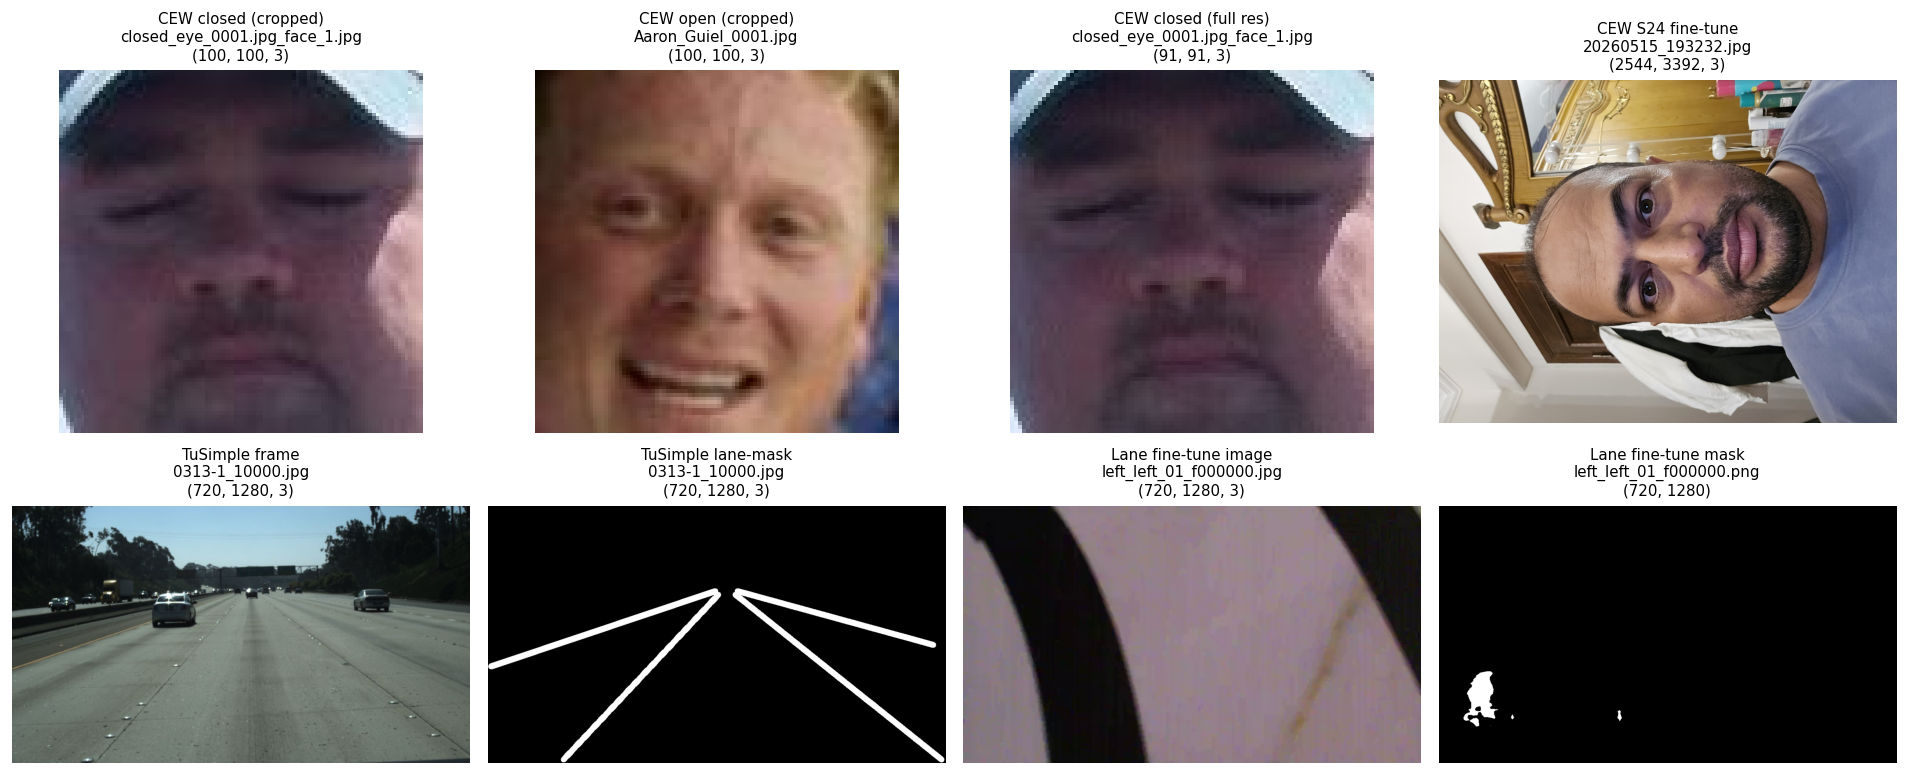
\includegraphics[width=\columnwidth]{fig_data_samples.png}
\caption{Eight-panel dataset sanity check. Top row, left to right:
CEW closed (cropped), CEW open (cropped), CEW closed (full-resolution),
CEW S24-Ultra fine-tune. Bottom row: TuSimple frame, TuSimple binary
lane-mask, lane fine-tune Pi-camera frame, lane fine-tune
SegFormer-regenerated road mask. The Pi-camera frame is visibly a
test-bench (dark tape on light cloth) rather than a real road, which
explains the very sparse SegFormer output beside it.}
\label{fig:data}
\end{figure}

\textbf{CEW (eye).} 2{,}423 cropped face images at
$100\!\times\!100$ (1{,}192 closed / 1{,}231 open). A deterministic
stratified $70/15/15$ split is persisted to
\texttt{artifacts/eye\_split.json} and is read verbatim by every
downstream notebook.

\textbf{TuSimple (lane).} 3{,}626 frames at $1280\!\times\!720$, split
at the \textit{clip} level (\texttt{cam\_seq}~$+$~\texttt{clip\_id}) to
prevent frame leakage. Direction labels are derived by fitting
$x = a y^2 + b y + c$ to the two ego-lane polylines, computing the
mean curvature coefficient~$a$, and bucketing $|a|$ at the 33rd and
67th percentile of the training distribution
($\tau \approx 1.96\!\times\!10^{-4}$). Frames with fewer than two
valid ego lanes are tagged as \textit{stop} for evaluation only.
Fig.~\ref{fig:lanepolys} shows three random TuSimple frames with the
polyline overlay and the cross-checked binary mask; this is the
ground-truth signal from which our direction labels are derived.
Fig.~\ref{fig:labelbal} plots the resulting class balance ($\sim$60\%
straight, $\sim$22\% right, $\sim$19\% left, $\sim$0\% naturally-stop)
---this imbalance drives the class-weighted training schedule and
later motivates the synthesized stop-class augmentation.

\begin{figure}[t]
\centering
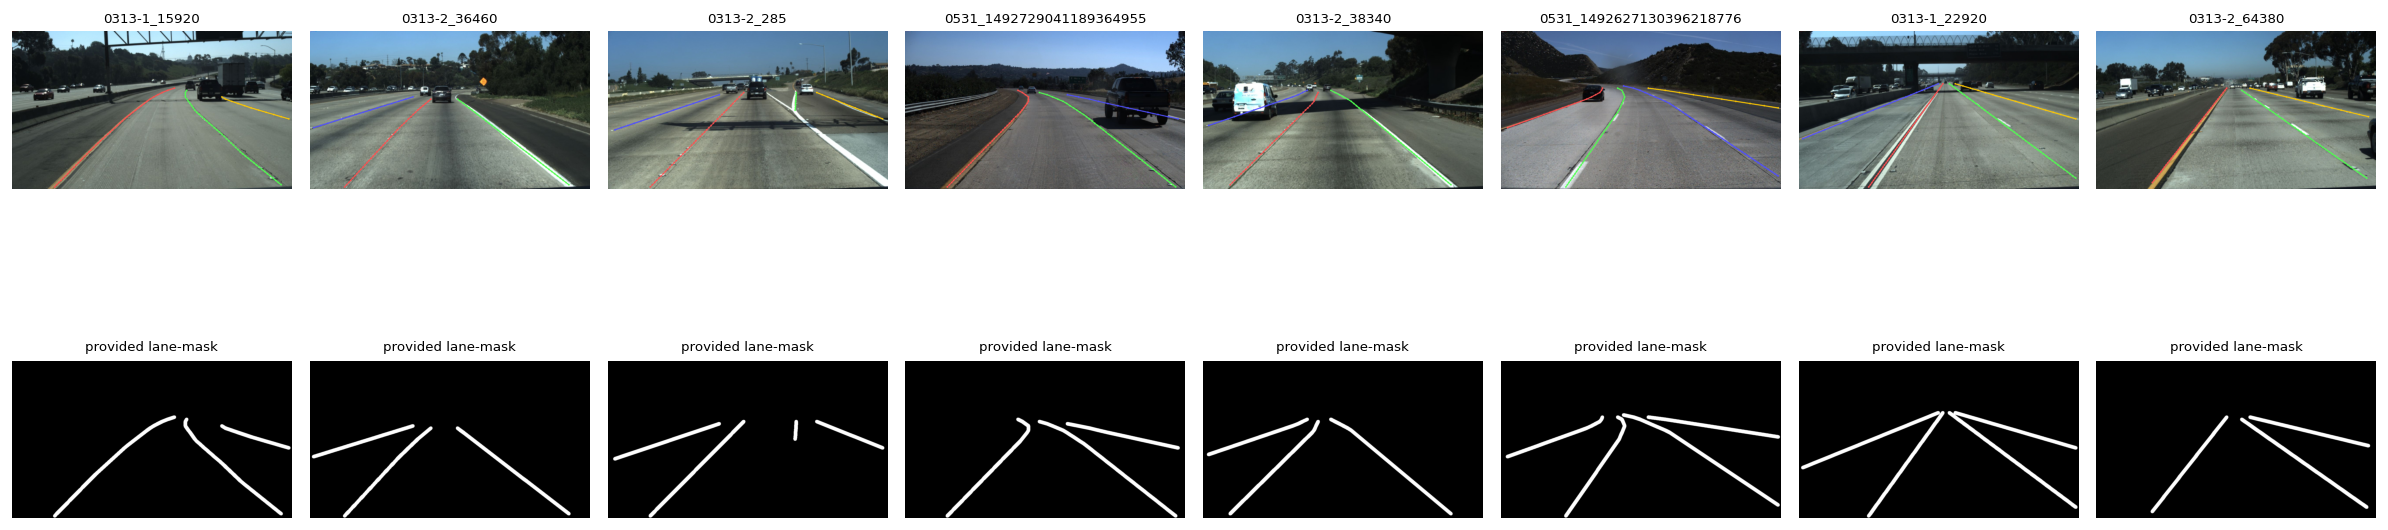
\includegraphics[width=\columnwidth]{fig_lane_polylines.png}
\caption{TuSimple frames with the four lane polylines overlaid (top
row) and the pre-rasterized binary lane mask (bottom row). The two
ego-lane polylines (typically green and blue) bracket the host
vehicle's lane; their average curvature drives our direction labels.}
\label{fig:lanepolys}
\end{figure}

\begin{figure}[t]
\centering
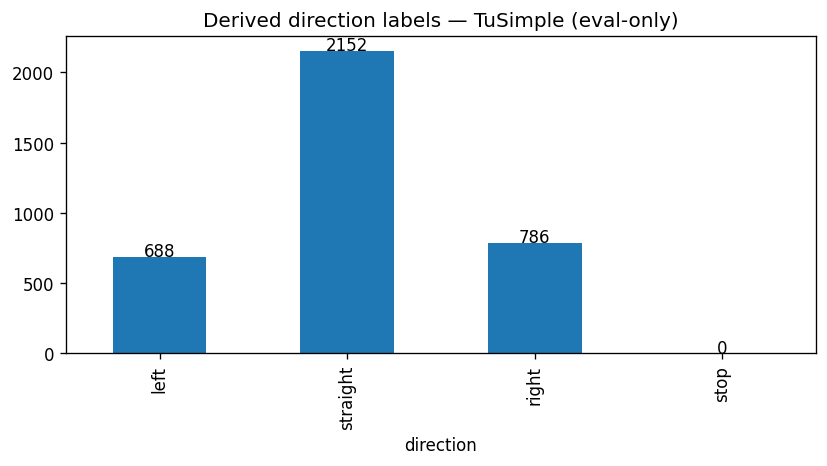
\includegraphics[width=0.7\columnwidth]{fig_lane_label_balance.png}
\caption{Derived four-class direction labels on the TuSimple
\textit{evaluation} subset. The stop class is essentially absent in
natural highway frames---we synthesize it at training time by zeroing
the lane region of a 10\% random subset.}
\label{fig:labelbal}
\end{figure}

\textbf{Pi fine-tune (lane).} 10{,}500 frames captured with the Pi
Camera~v2, balanced 3{,}500 per direction class after augmentation.
Binary road masks are regenerated with
SegFormer-B2-cityscapes \cite{segformer} as a visual aid; the lane
classifier itself consumes RGB only.

\textbf{Phone fine-tune (eye).} 12 full-frame portraits captured on
the S24~Ultra; the two displayed in Fig.~\ref{fig:phonedetect}
(\textit{author's own face, eyes-open / eyes-closed pair}) are shown
here as a representative sample for privacy reasons---the remaining
ten frames involve other people and are used internally by the
fine-tune notebook but not reproduced in this paper. All captures are
full-face photographs in landscape orientation, so eye/07 first
rotates them to portrait via a four-rotation face-detection vote, then
crops the detected face to $100\!\times\!100$ to match the CEW domain
before any fine-tune step.

\begin{figure}[t]
\centering
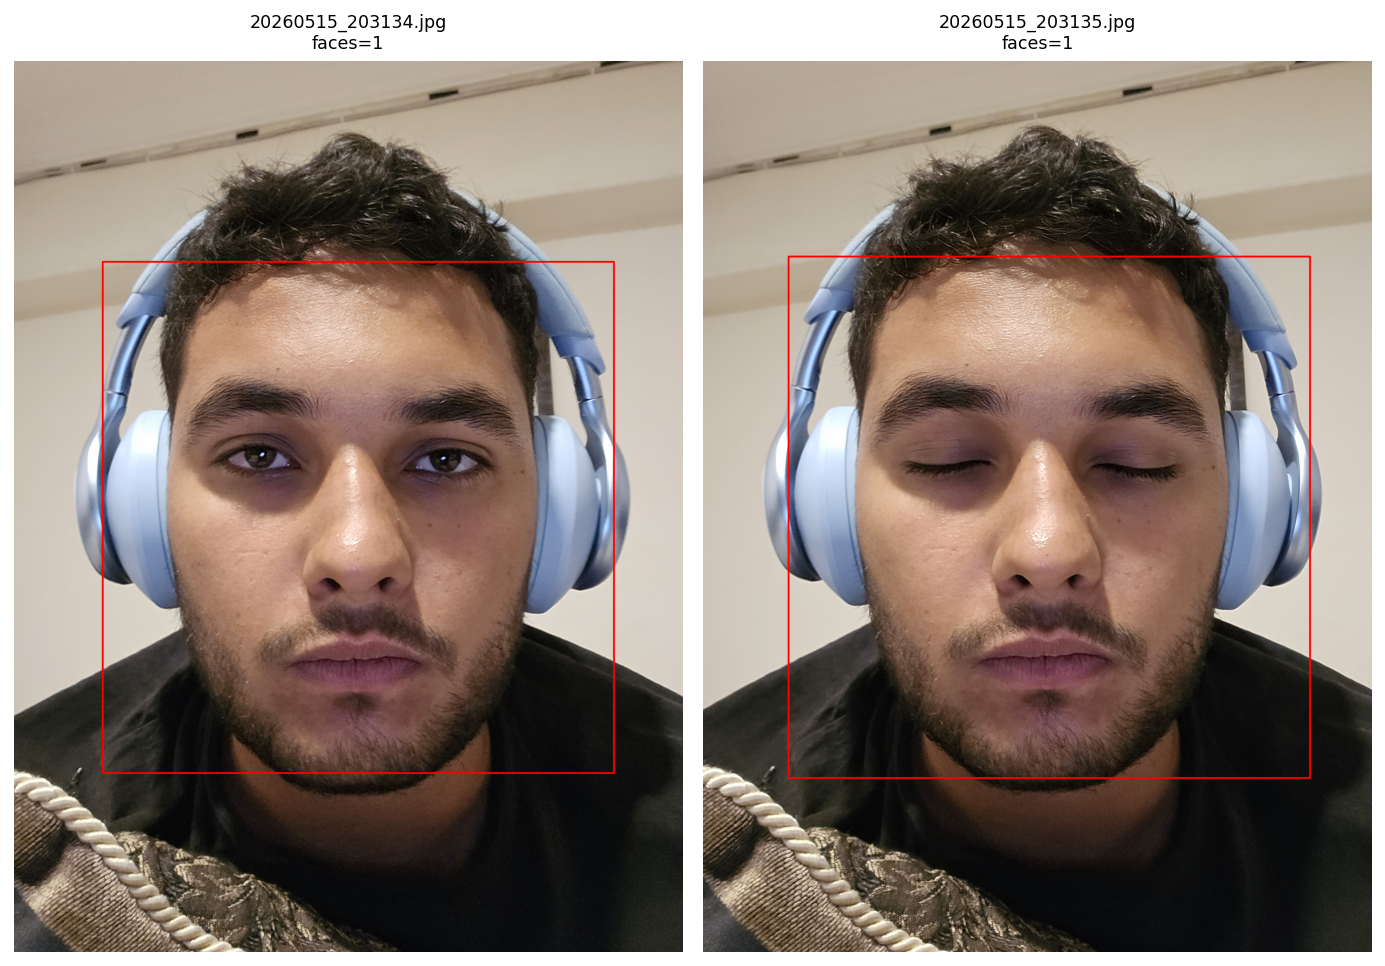
\includegraphics[width=0.75\columnwidth]{fig_eye_phone_detect.png}
\caption{Representative S24-Ultra fine-tune pair (open / closed) for
one subject (the author), after orientation correction and Haar face
detection. The pipeline correctly locates the largest face in both
frames despite landscape capture and the headphones; the same
behavior holds for the other ten captures, which are omitted from
this figure for privacy.}
\label{fig:phonedetect}
\end{figure}

\subsection{Reproducibility}
All notebooks fix \texttt{random}, \texttt{numpy}, \texttt{torch}, and
\texttt{tensorflow} seeds to 42 in their first code cell, exactly
mirroring \texttt{notebooks/00\_setup\_environment.ipynb}. Splits are
JSON files; manifests of measured numbers are JSON files; figures are
PNGs regenerated from those JSON files by
\texttt{notebooks/09\_paper\_figures.ipynb}.

\subsection{Classical baselines}

\textbf{Eye.} Grayscale + CLAHE, HOG ($8\!\times\!8$ pixels-per-cell,
$2\!\times\!2$ cells-per-block, 9 orientations), and a linear SVM with
grid-searched $C$. Fig.~\ref{fig:eyeclassical} shows the staged
output: from the raw $100\!\times\!100$ face crop, through CLAHE, to
the Canny edge map and HOG visualization. The HOG cells around the
eye sockets carry the discriminative signal that the SVM ultimately
keys on.

\begin{figure}[t]
\centering
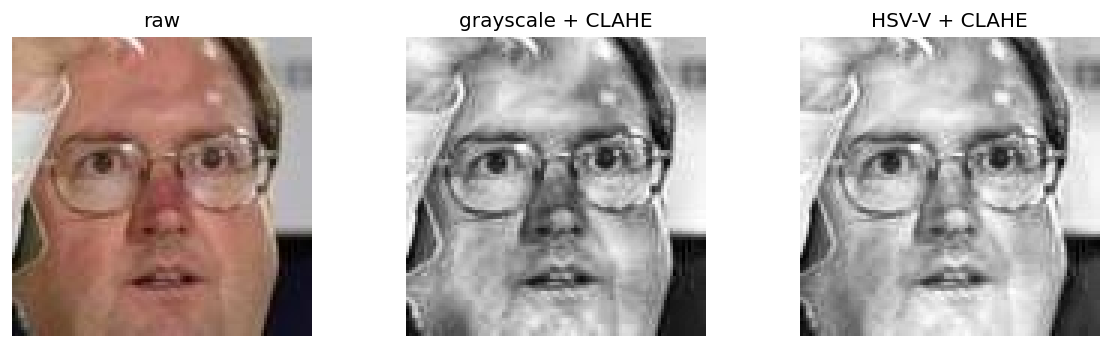
\includegraphics[width=\columnwidth]{fig_eye_classical.png}
\caption{Eye classical pipeline staged on one CEW sample: raw crop
$\rightarrow$ grayscale~$+$~CLAHE $\rightarrow$ Otsu-adaptive Canny
edges $\rightarrow$ HOG visualization. The localized eye-region
gradients dominate the HOG response, which is what the linear SVM
ultimately classifies.}
\label{fig:eyeclassical}
\end{figure}

\textbf{Lane.} ROI cropping to the lower 60\% of a downsampled
$640\!\times\!360$ frame, an HSV-saturation $+$ grayscale fused
channel, Canny, probabilistic Hough lines clustered into left and
right groups by slope sign, and a 30-D feature vector (per-side line
statistics + 12-bin angle histogram) fed to a one-vs-rest linear SVM.
Fig.~\ref{fig:lanehough} visualizes the edge map and the resulting
classified lines on a representative TuSimple frame. Lines with
negative slope (red) form the left lane group, positive slope (green)
the right; the SVM uses the per-group statistics rather than any
individual line.

\begin{figure}[t]
\centering
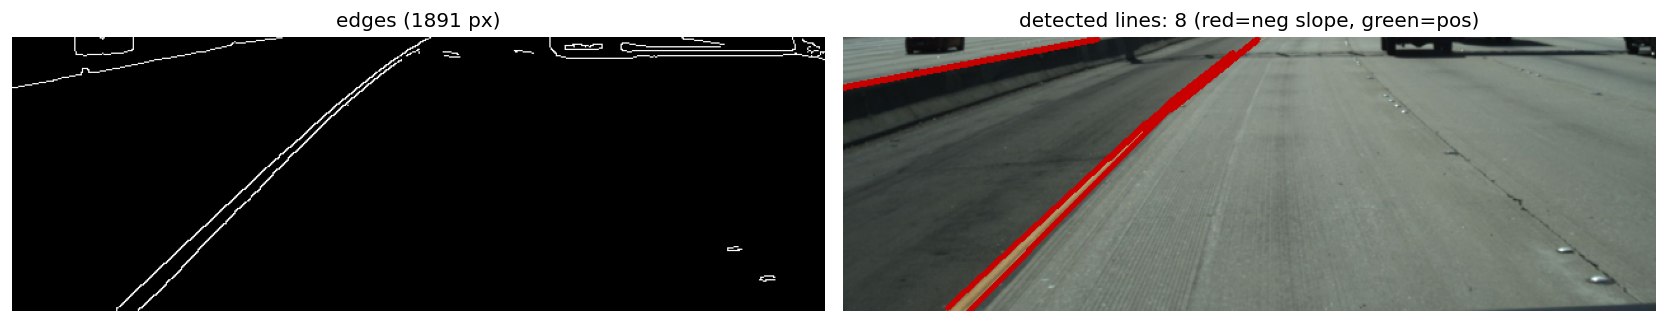
\includegraphics[width=\columnwidth]{fig_lane_hough.png}
\caption{Lane classical pipeline: Canny edge map (left) and detected
probabilistic Hough lines (right) on a TuSimple frame. Red = negative
slope (left-side candidates), green = positive slope (right-side
candidates); the SVM operates on aggregated per-side statistics, not
individual lines.}
\label{fig:lanehough}
\end{figure}

\subsection{Custom CNN (from scratch)}

Both pipelines train a small \textit{Conv $\rightarrow$ BN $\rightarrow$
ReLU $\rightarrow$ MaxPool} stack ending in GAP + Dropout + Dense. The
eye model uses widths $(16, 32, 64)$ on $64\!\times\!64$ grayscale
input ($\sim$25.8\,k parameters); the lane model uses widths
$(16, 32, 64, 96)$ on $128\!\times\!128$ RGB input ($\sim$86.3\,k
parameters). Neither uses pretrained weights, per the project rubric.

\subsection{Dedicated transfer-learning notebook}
Per the approved plan, transfer learning lives in its own notebook
(\texttt{eye/04} and \texttt{lane/04}), evaluating four candidates per
pipeline: MobileNetV2 and MobileNetV3-Small (ImageNet) $\times$
\{frozen, fine-tune\}. The lane TL notebook was originally planned
around a MobileNetV2$+$UFLDv2 row-anchor head; the absence of usable
road masks in the Pi-camera domain (Section~\ref{sec:discussion})
prompted us to replace the row-anchor head with a standard
classification head while keeping the MobileNetV2 backbone.

\subsection{Experimental study (one variable at a time)}
Each pipeline runs four controlled experiments against its
from-scratch baseline: \textbf{(A)} data augmentation
(none / light / heavy), \textbf{(B)} color space
(RGB / grayscale / HSV), \textbf{(C)} robustness under synthetic
distortions (test-time only: Gaussian noise $\sigma{\in}\{15,25\}$,
motion-blur $k{=}15$, brightness $\pm 40\%$, fog $\alpha{=}0.4$,
$25\%$ ROI occlusion), and \textbf{(D)} lightweight design
(tiny depthwise-separable / baseline / wider). Each experiment uses
the same seed, same split, same metric set.

\subsection{Model selection}
For every candidate produced by Notebooks 02--05 we record clean
accuracy, macro-F1, robust accuracy, parameter count and the int8
TFLite size. A weighted score
\begin{align}
\text{eye score}\;&=\;0.35\,a\;+\;0.20\,a_r\;+\;0.15\,f\nonumber\\
                  &\;\;+\;0.15(1-\hat\ell)\;+\;0.10(1-\hat s)\;+\;0.05(1-\hat p)\\
\text{lane score}\;&=\;0.25\,a\;+\;0.20\,f\;+\;0.15\,a_r\nonumber\\
                   &\;\;+\;0.25(1-\hat\ell)\;+\;0.10(1-\hat s)\;+\;0.05(1-\hat p)
\end{align}
combines clean accuracy $a$, macro-F1 $f$, robust accuracy $a_r$, and
min-max-normalized latency $\hat\ell$, size $\hat s$ and parameters
$\hat p$. The eye weights tilt toward accuracy (NPU-class hardware
target), while the lane weights tilt toward latency (no NPU on the
Pi). For each pipeline we also extract the Pareto frontier on the
accuracy-vs-parameters plane, so the choice remains defensible if a
reviewer disagrees with the weighting.

\subsection{Deployment}
The eye winner is converted to four TFLite variants (FP32, PTQ-int8,
QAT-int8 when TFMOT is available) and the int8 model is benchmarked
on a real Samsung~S24~Ultra (SM-S928B, Snapdragon~8~Gen~3, Adreno~750
GPU, Hexagon NPU) using the official TFLite Benchmark APK across the
CPU (XNNPACK, 4 threads), GPU (Adreno OpenCL) and NNAPI delegates.
The lane winner is exported to FP32 and PTQ-int8 TFLite, plus an
OpenVINO ARM-CPU IR; on-device latency on the Pi~4B is reported as a
\emph{simulated} estimate calibrated against published RPi benchmarks
until a real device is available.

% ============================================================================
\section{Experiments and Results}\label{sec:results}

\subsection{Eye pipeline}

\textbf{Custom CNN training behavior.}
Fig.~\ref{fig:eyetrain} shows the eye CNN's training and validation
curves. The model converges within ten epochs and the
train/validation gap remains modest ($<$0.05 across all epochs),
indicating that the dropout (0.5) and global-average-pooling head
provide sufficient regularization at this dataset scale. The
characteristic ``L'' shape of the validation loss---fast drop in the
first five epochs followed by an oscillating plateau---is consistent
with the EarlyStopping cut-off at epoch 30.

\begin{figure}[t]
\centering
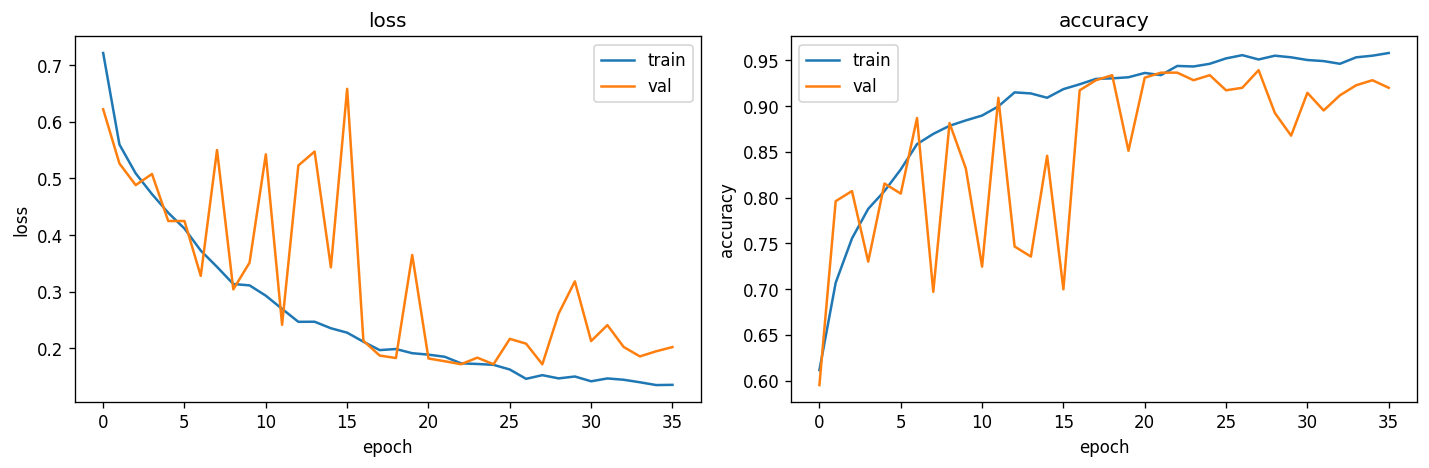
\includegraphics[width=\columnwidth]{fig_eye_train.png}
\caption{Eye custom CNN: training and validation loss/accuracy across
30 epochs. The narrow train-val gap confirms that overfitting is
controlled at the chosen 25.8\,k-parameter capacity.}
\label{fig:eyetrain}
\end{figure}

\textbf{Eye CNN confusion and ROC.}
The confusion matrix in Fig.~\ref{fig:eyecm} is symmetric and slightly
favors recall on the \textit{open} class. The ROC AUC of $\sim$0.96
demonstrates that the model is well-calibrated; the small residual
errors concentrate on partially-open eyes that fall on the decision
boundary.

\begin{figure}[t]
\centering
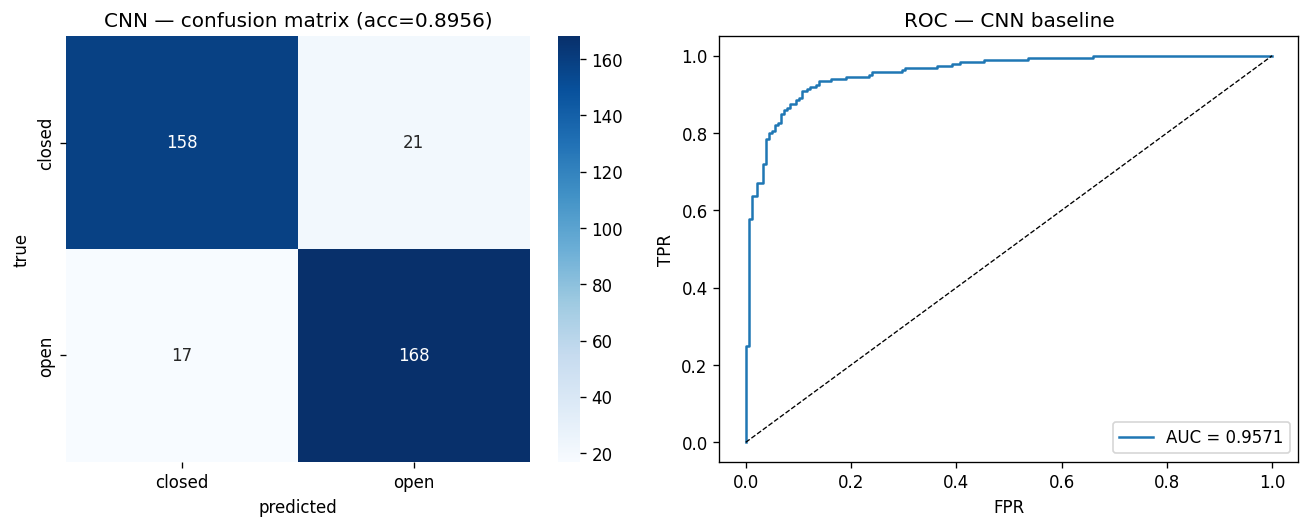
\includegraphics[width=\columnwidth]{fig_eye_cm_roc.png}
\caption{Eye custom CNN: confusion matrix (left) and ROC curve
(right) on the CEW test split.}
\label{fig:eyecm}
\end{figure}

\textbf{Transfer-learning behavior.}
Fig.~\ref{fig:eyetl} overlays the validation curves of all four
TL candidates against the from-scratch CNN. The MobileNetV2 candidates
converge quickly but plateau below the from-scratch model; the V3-Small
candidates require more epochs and never catch up. The
parameter-vs-accuracy plot in Fig.~\ref{fig:eyepa} makes the
inefficiency explicit: at any fixed accuracy point above $0.85$,
the from-scratch CNN uses roughly two orders of magnitude fewer
parameters than the corresponding TL candidate.

\begin{figure}[t]
\centering
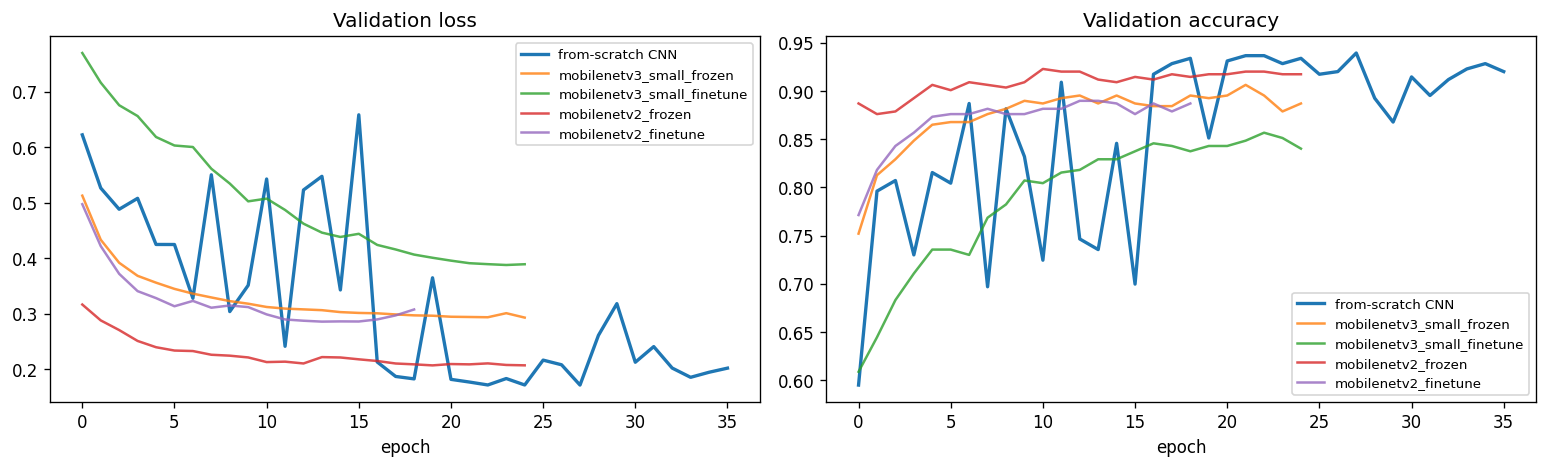
\includegraphics[width=\columnwidth]{fig_eye_tl_curves.png}
\caption{Eye transfer-learning candidates compared with the
from-scratch CNN (black dashed). Even the best TL candidate
(MobileNetV2-finetune) does not exceed the from-scratch model on
CEW.}
\label{fig:eyetl}
\end{figure}

\begin{figure}[t]
\centering
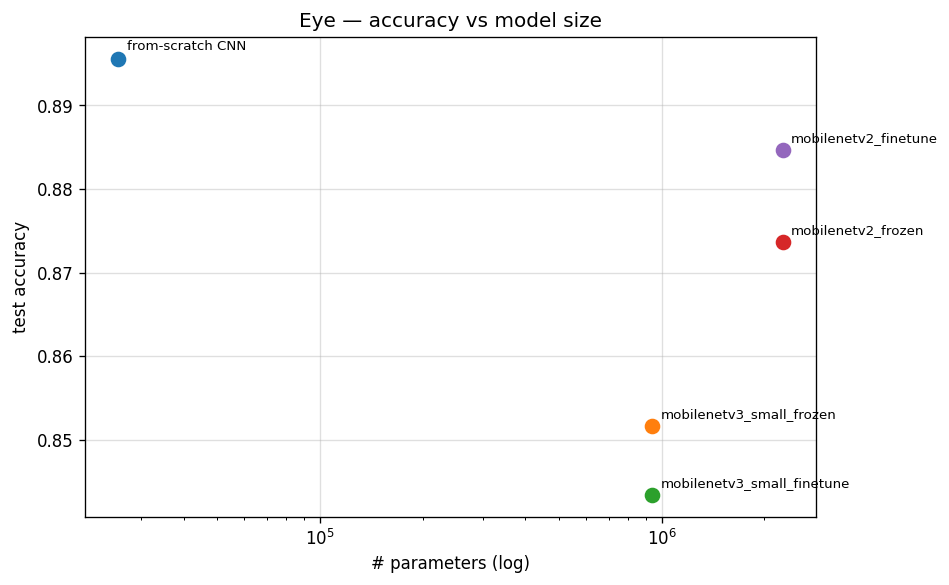
\includegraphics[width=0.95\columnwidth]{fig_eye_params_acc.png}
\caption{Eye transfer-learning candidates plotted on parameter count
(log scale) vs.\ test accuracy. The from-scratch CNN (black square)
dominates all four MobileNet variants on both axes.}
\label{fig:eyepa}
\end{figure}

\textbf{Augmentation, color, and lightweight studies.}
Fig.~\ref{fig:eyeABD} shows the three controlled-variable experiments
that do not involve transfer learning. \emph{Light} augmentation
(horizontal flip + $\pm 10\circ$ rotation + brightness) yields the
biggest single-variable jump in accuracy; heavy augmentation overshoots
and slightly degrades performance, indicating that aggressive cutout
and elastic deformation are too far from CEW's distribution to help.
Color space matters very little---all three of RGB, grayscale, and HSV
land within $\pm 0.01$ of one another, validating the grayscale
preprocessing chosen for the classical pipeline. The lightweight
sweep finds the sweet spot at the \textit{wide} variant
($\sim$97\,k parameters): the tiny variant ($\sim$4\,k parameters) is
under-capacity, while the wider variant gains both accuracy and a
better quantization tolerance.

\begin{figure}[t]
\centering
\subfloat[Exp-A augmentation]{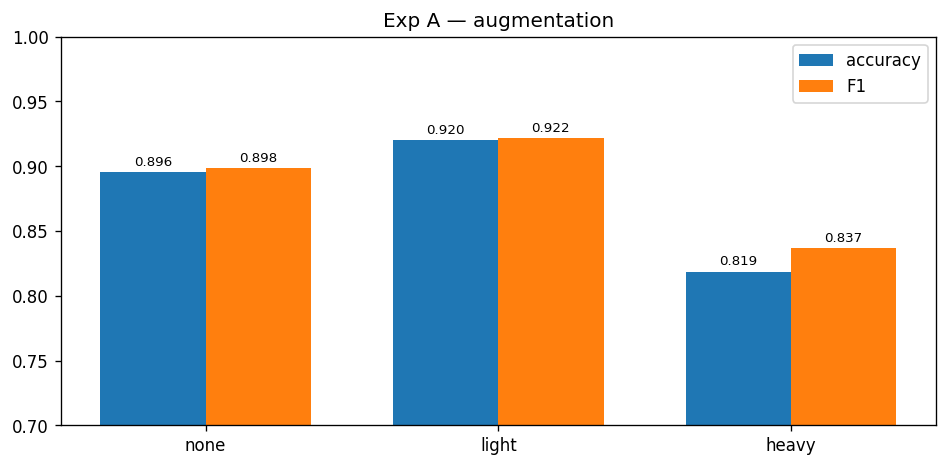
\includegraphics[width=0.32\columnwidth]{fig_eye_expA.png}}\hfill
\subfloat[Exp-B color space]{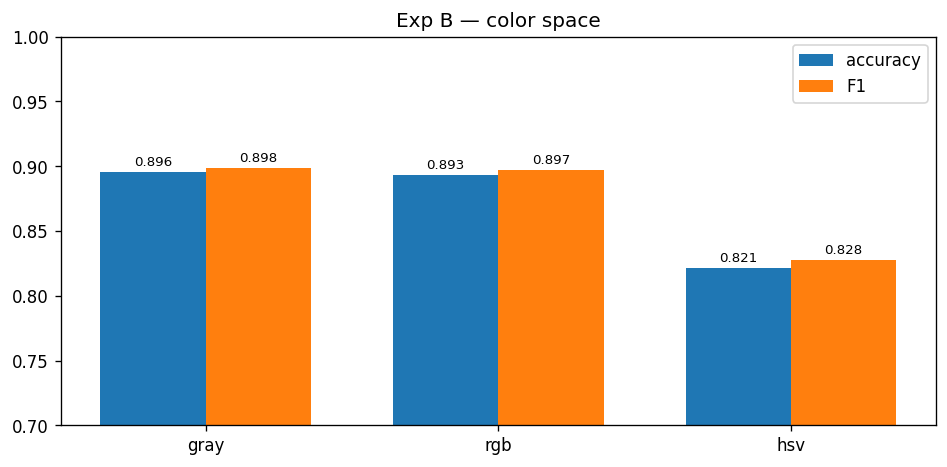
\includegraphics[width=0.32\columnwidth]{fig_eye_expB.png}}\hfill
\subfloat[Exp-D lightweight]{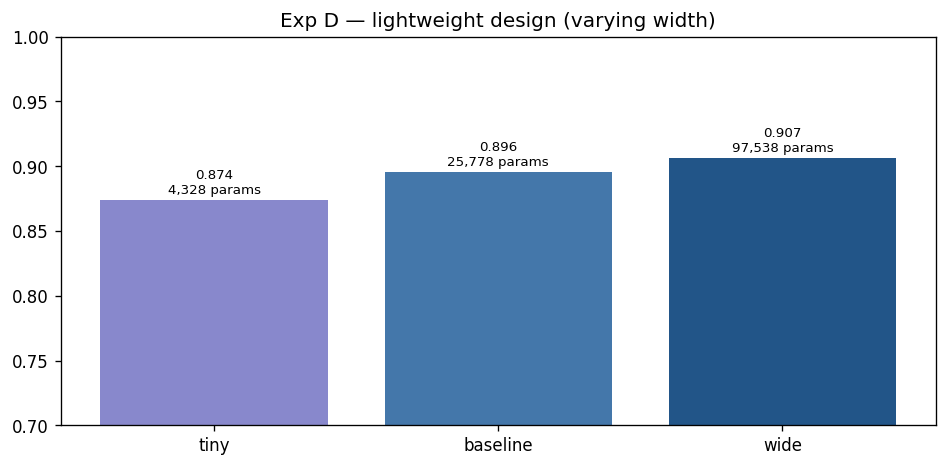
\includegraphics[width=0.32\columnwidth]{fig_eye_expD.png}}
\caption{Eye controlled-variable experiments. Light augmentation
helps; color space is nearly indifferent; the \textit{wide} lightweight
variant wins.}
\label{fig:eyeABD}
\end{figure}

\textbf{Robustness.}
Fig.~\ref{fig:eyerobust} shows the eye CNN's accuracy under the
distortion suite. Brightness shifts and motion blur are the dominant
failure modes ($-$0.15--0.25 accuracy); Gaussian noise is relatively
benign because CEW images are themselves grainy. Mean robust accuracy
across the suite is $0.662$.

\begin{figure}[t]
\centering
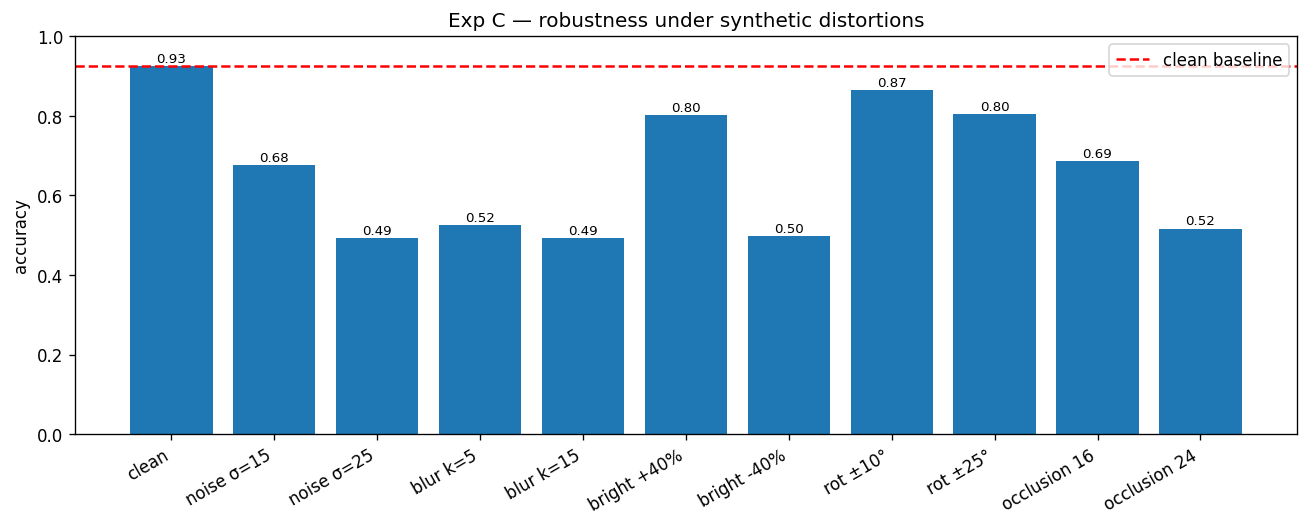
\includegraphics[width=\columnwidth]{fig_eye_robust.png}
\caption{Eye from-scratch CNN under the synthetic-distortion suite.
The clean reference is the leftmost bar; degradations are
substantial for motion blur and brightness extremes.}
\label{fig:eyerobust}
\end{figure}

\textbf{Eye misclassification gallery.}
Fig.~\ref{fig:eyemisses} shows the eight worst-confidence
misclassifications from the test set. They are dominated by
half-closed or sideways-glance eyes, exactly the boundary cases the
binary framing cannot disambiguate. A future three-class
``open / half / closed'' formulation would likely absorb these errors.

\begin{figure}[t]
\centering
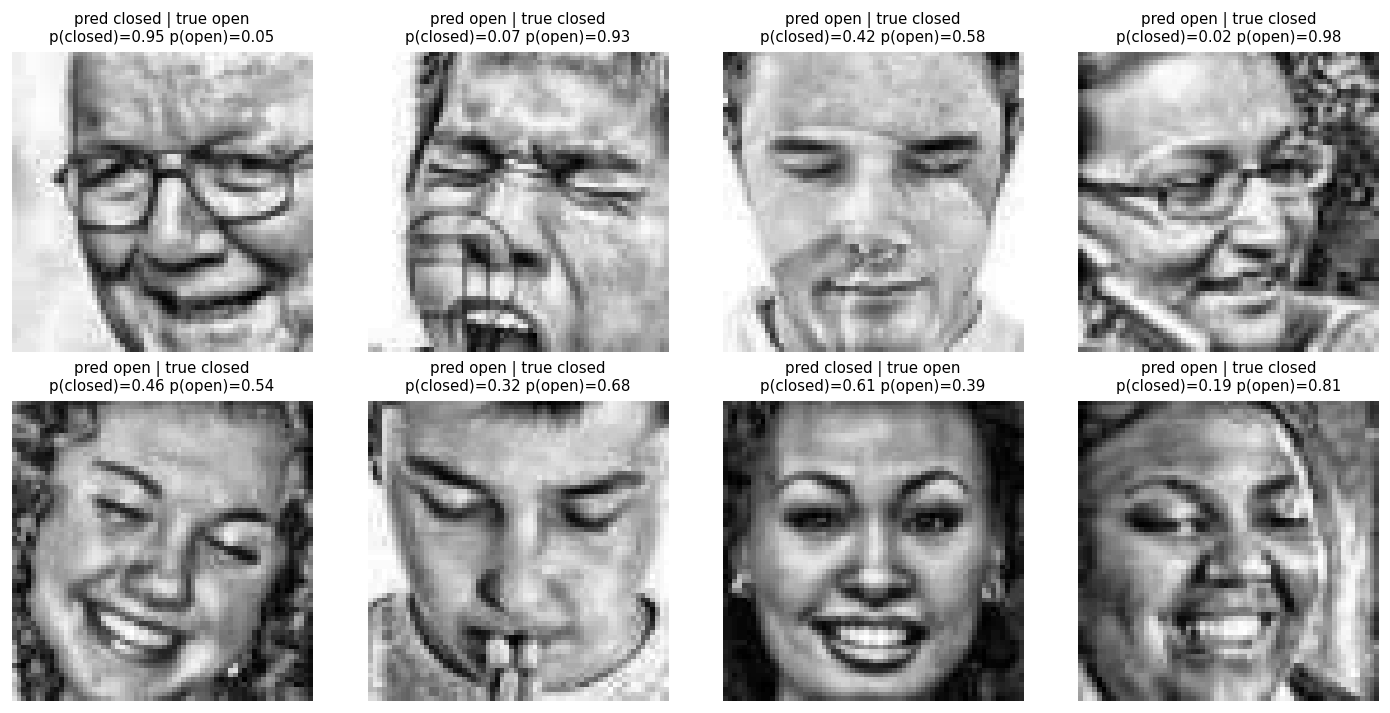
\includegraphics[width=\columnwidth]{fig_eye_misses.png}
\caption{Eight highest-confidence misclassifications by the eye CNN.
The dominant failure mode is partially-open or sideways-glance eyes
on which the binary frame is structurally ambiguous.}
\label{fig:eyemisses}
\end{figure}

\textbf{Final eye selection.}
Table~\ref{tab:eye} consolidates every candidate that fed the
model-selection algorithm. The Pareto frontier in Fig.~\ref{fig:pareto}
(left panel) confirms that the lightweight family dominates all of
the parameter-axis until $\sim$10\,M parameters, where the
MobileNet variants finally appear---and even there they do not exceed
the wide-lightweight accuracy. The weighted-score winner is therefore
\textit{lw\_wide} at 97\,k parameters, $0.907$ accuracy, $0.091$\,MB
int8.

\begin{table}[t]
\centering
\caption{Eye pipeline candidates (CEW test split, $N{=}364$).}
\label{tab:eye}
\begin{tabular}{lcccr}
\toprule
Model & Acc. & F1 & Params & Family\\
\midrule
classical HOG+SVM         & 0.874 & 0.876 & 14\,k   & classical\\
cnn\_from\_scratch        & 0.896 & 0.898 & 25\,778 & CNN\\
mobilenetv3\_small\_frozen   & 0.852 & 0.859 & 940\,274  & TL\\
mobilenetv3\_small\_finetune & 0.843 & 0.847 & 940\,274  & TL\\
mobilenetv2\_frozen          & 0.874 & 0.872 & 2{,}260\,546 & TL\\
mobilenetv2\_finetune        & 0.885 & 0.888 & 2{,}260\,546 & TL\\
lw\_tiny                  & 0.874 & 0.873 & 4\,328  & lightweight\\
lw\_baseline              & 0.896 & 0.898 & 25\,778 & lightweight\\
\textbf{lw\_wide $\,\star$} & \textbf{0.907} & \textbf{0.910} & 97\,538 & lightweight\\
\bottomrule
\end{tabular}
\end{table}

\begin{figure}[t]
\centering
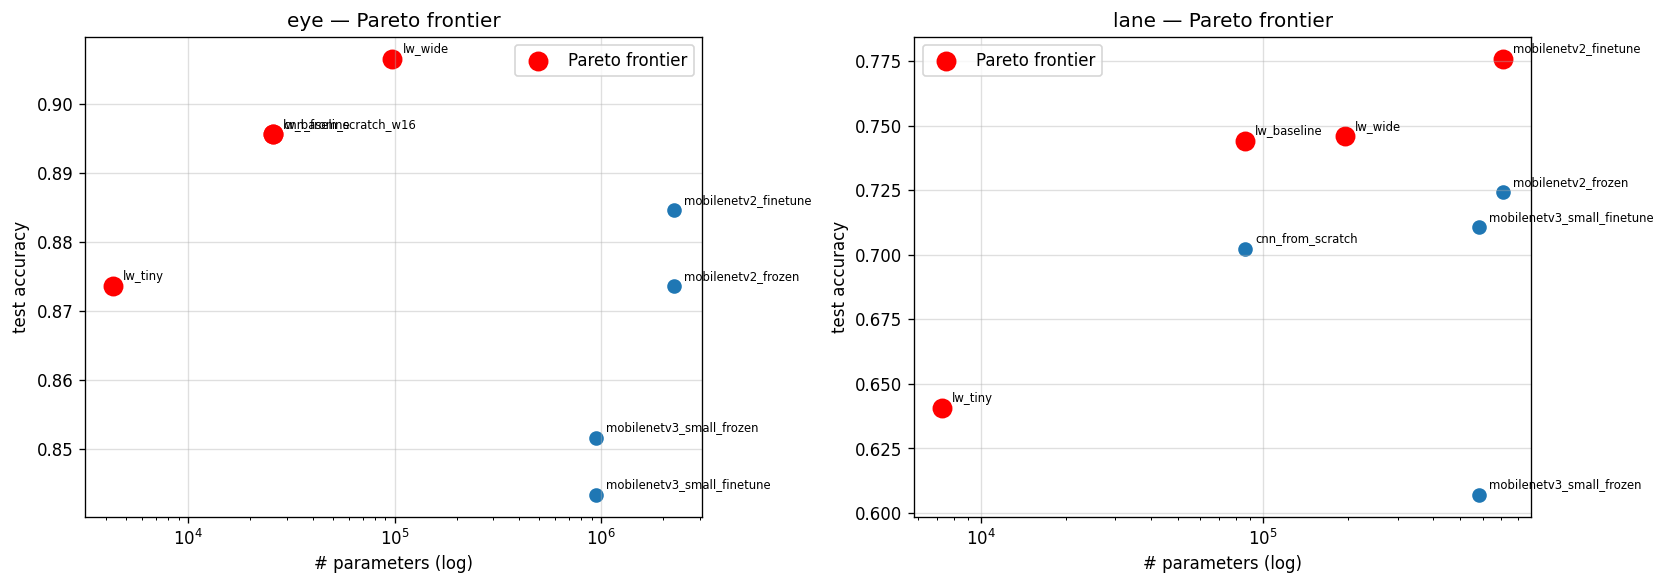
\includegraphics[width=\columnwidth]{fig_pareto.png}
\caption{Pareto frontiers for the eye pipeline (left) and the lane
pipeline (right). Pareto-optimal candidates are highlighted in red.}
\label{fig:pareto}
\end{figure}

\subsection{Lane pipeline}

\textbf{Lane CNN training and confusion.}
Fig.~\ref{fig:lanetrain} plots the lane CNN's training curves.
EarlyStopping fires at epoch~21, with a final train accuracy of
$0.822$ against a validation accuracy of $0.694$. The
class-weighted loss is essential here: without it, the
straight-dominant TuSimple distribution causes the network to collapse
to the majority class. Fig.~\ref{fig:lanecnncm} shows the resulting
four-class confusion matrix---the model correctly identifies the
synthesized \textit{stop} class with $100\%$ recall but confuses
roughly half of the gentle left/right curves with \textit{straight},
which is the expected and hardest case.

\begin{figure}[t]
\centering
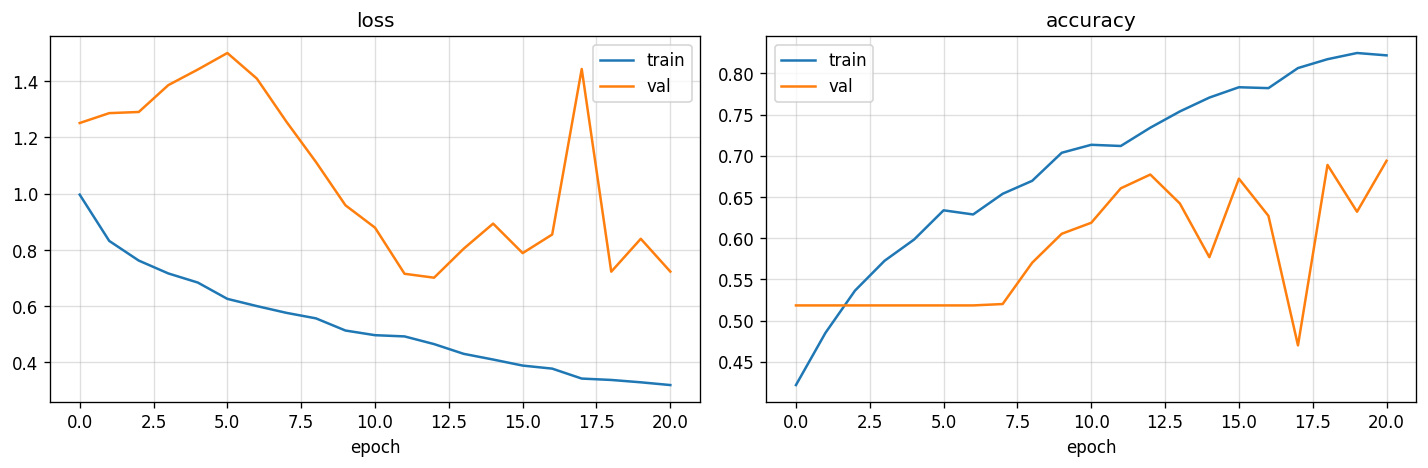
\includegraphics[width=\columnwidth]{fig_lane_train.png}
\caption{Lane custom CNN: training/validation curves. The 0.13
train-val gap is the largest of the project, reflecting the heavier
distortion of the lane task.}
\label{fig:lanetrain}
\end{figure}

\begin{figure}[t]
\centering
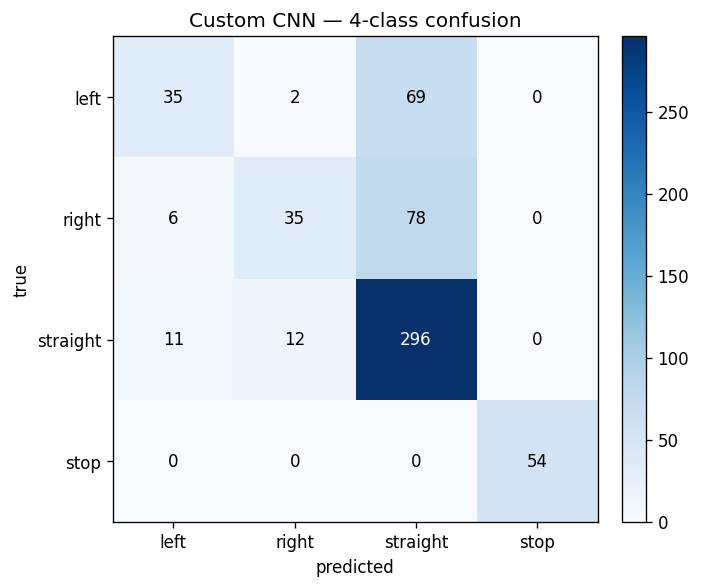
\includegraphics[width=0.7\columnwidth]{fig_lane_cnn_cm.png}
\caption{Lane custom CNN: four-class confusion matrix on the TuSimple
test split. The synthesized stop class is perfectly separable; the
dominant remaining error is gentle curves predicted as straight.}
\label{fig:lanecnncm}
\end{figure}

\textbf{Lane misclassification gallery.}
Fig.~\ref{fig:lanemisses} confirms the conclusion from the confusion
matrix: the failures are visually plausible---frames where the
curvature is subtle, where there is glare, or where the second-most-
relevant lane is partly occluded by another vehicle. These are the
same failure modes that motivate post-processing with temporal
smoothing in a deployed system.

\begin{figure}[t]
\centering
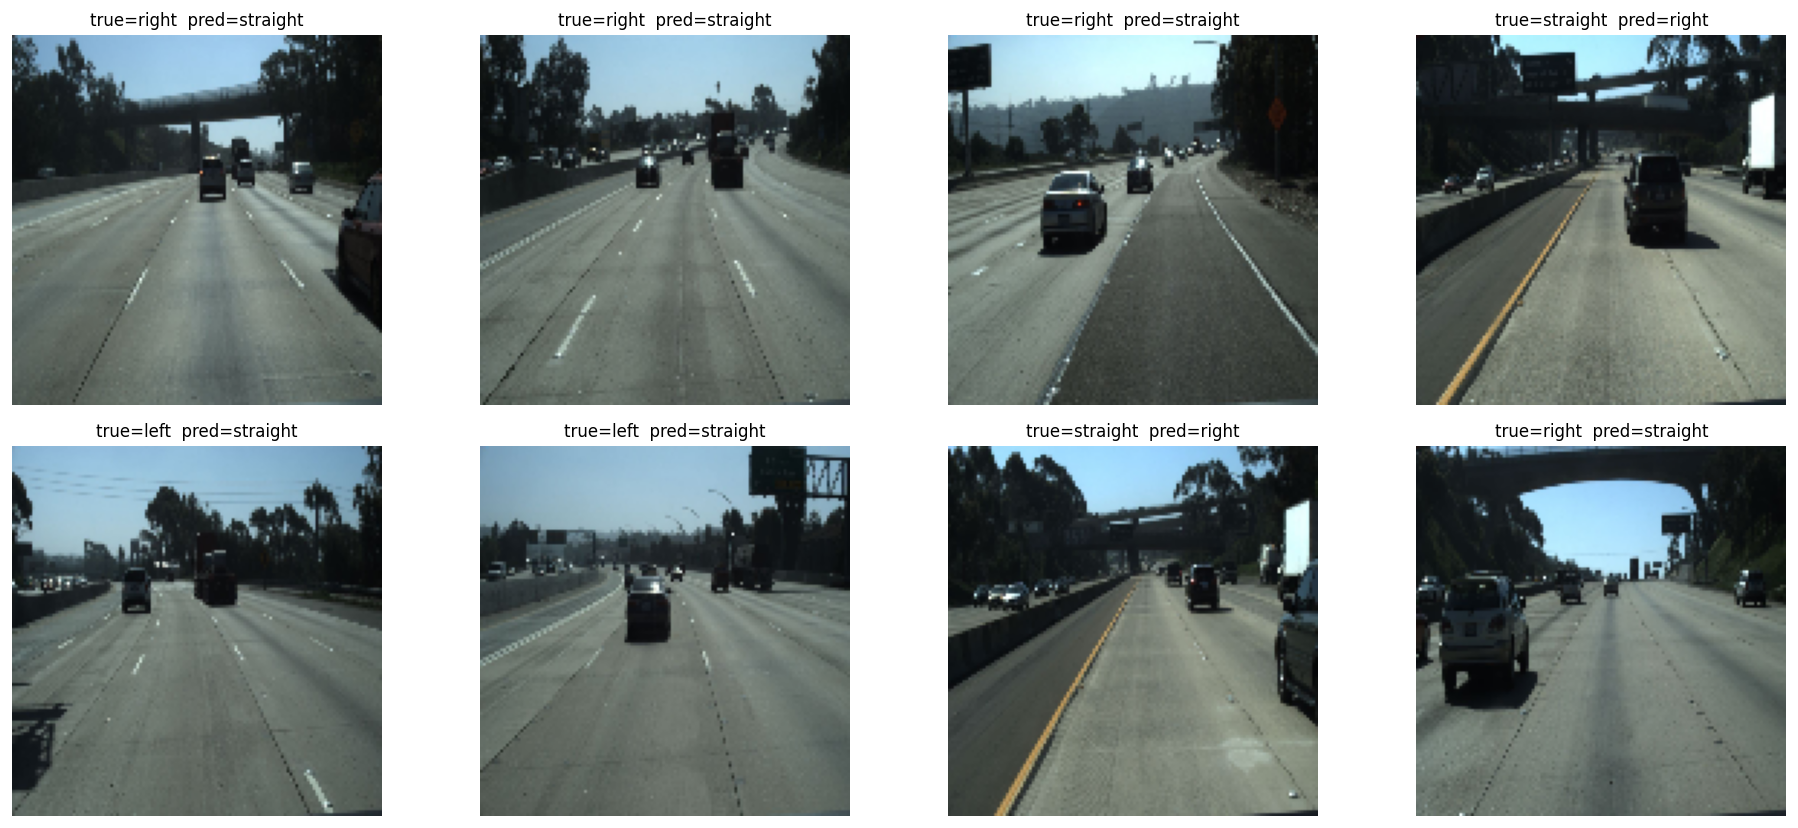
\includegraphics[width=\columnwidth]{fig_lane_misses.png}
\caption{Eight worst lane CNN test misclassifications. All eight are
gentle-curve frames mislabeled as straight, on roads where a single
frame is in fact ambiguous to a human observer.}
\label{fig:lanemisses}
\end{figure}

\textbf{Lane transfer-learning comparison.}
Fig.~\ref{fig:lanetlcurves} overlays the validation curves of all four
TL candidates against the lane CNN. Unlike the eye pipeline, the lane
TL candidates \emph{do} outperform the from-scratch CNN
(MobileNetV2-finetune reaches $0.776$ vs.\ $0.702$), because the
TuSimple task has more visual richness than the CEW eye-state task.
The four confusion matrices in Fig.~\ref{fig:lanetlcms} show that the
gain comes mostly from better discrimination between left and right
curves; the straight column remains the most over-predicted in every
candidate.

\begin{figure}[t]
\centering
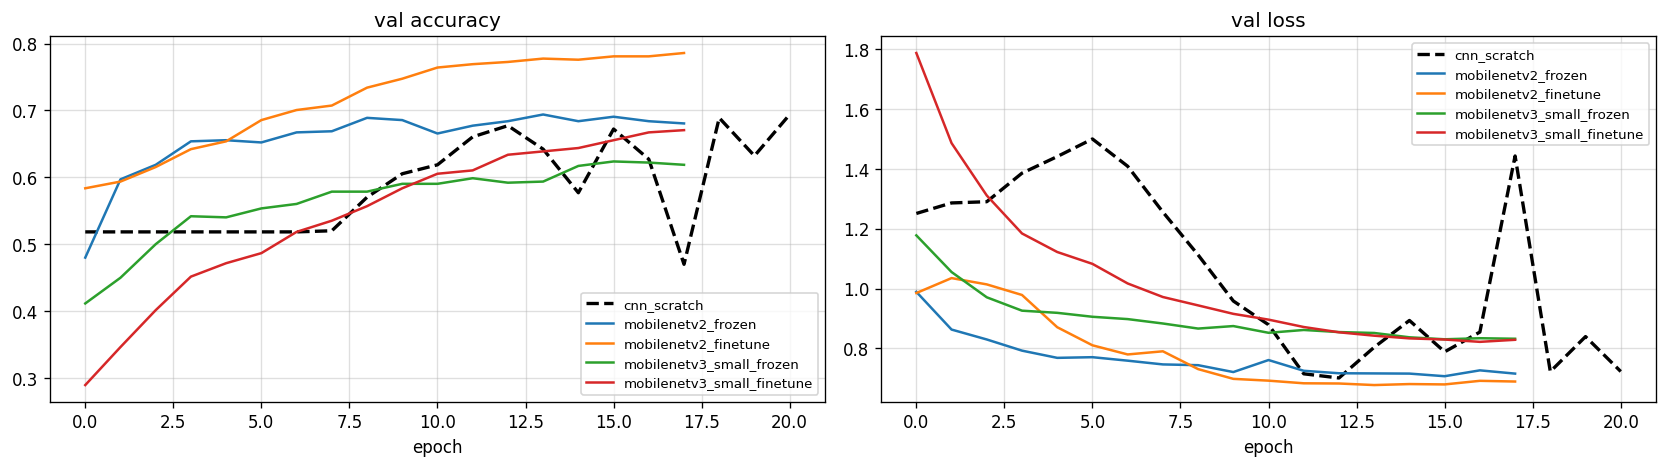
\includegraphics[width=\columnwidth]{fig_lane_tl_curves.png}
\caption{Lane TL candidates vs.\ from-scratch CNN (black dashed). On
TuSimple, transfer learning does help: MobileNetV2-finetune sits 7\,pp
above the from-scratch baseline.}
\label{fig:lanetlcurves}
\end{figure}

\begin{figure}[t]
\centering
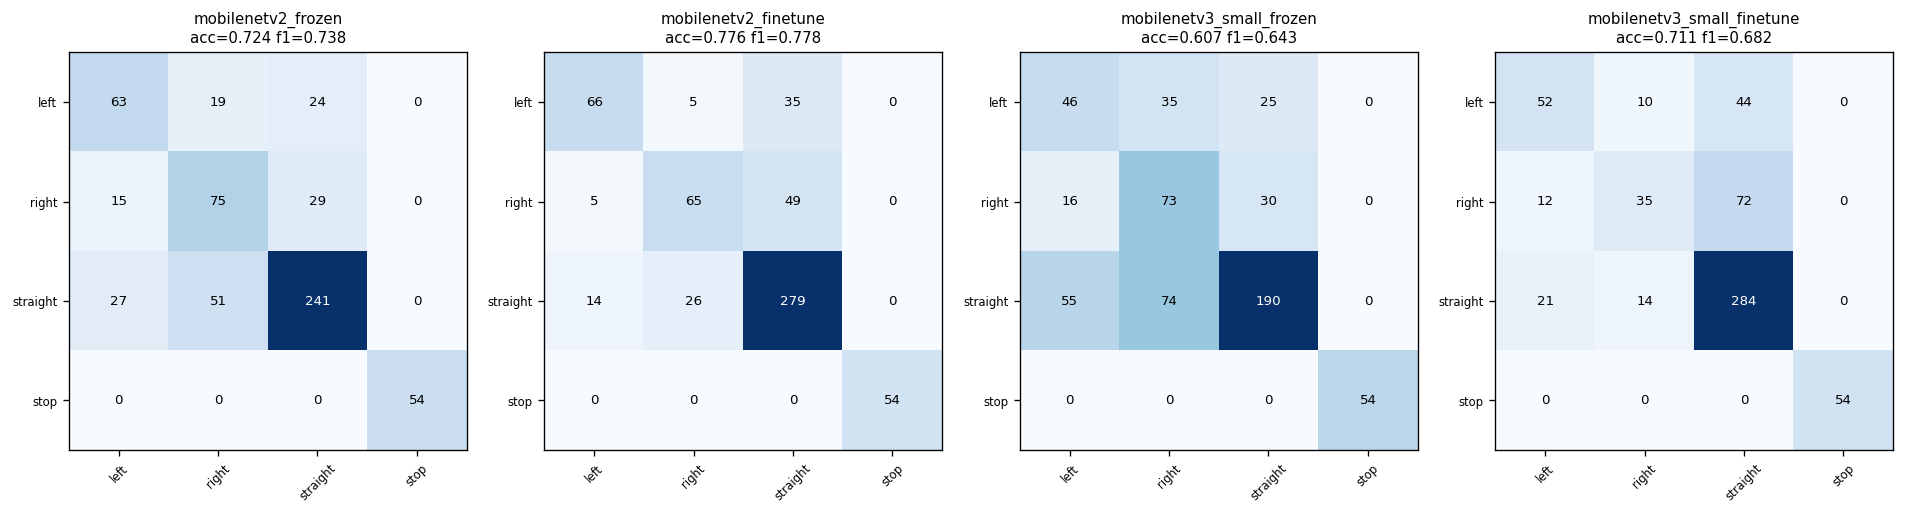
\includegraphics[width=\columnwidth]{fig_lane_tl_cms.png}
\caption{Confusion matrices of the four lane TL candidates. The gain
over the from-scratch CNN is concentrated in left/right discrimination.}
\label{fig:lanetlcms}
\end{figure}

\textbf{Lane experiments.}
Fig.~\ref{fig:laneABD} reports the augmentation and lightweight
studies on the lane pipeline. The augmentation finding is striking:
without augmentation the model collapses to the majority class, with
light augmentation it recovers to $0.69$, with heavy augmentation it
recovers to $0.66$. Color space results (not shown for brevity) are
similar to the eye finding---all three of RGB / gray / HSV land
within $\pm 0.02$ of one another after the recovery procedure
described in Section~\ref{sec:discussion}. The lightweight sweep
selects the \textit{baseline} variant ($\sim$86\,k parameters) because
the wider variant fails to amortize its extra weights on the
TuSimple-sized dataset.

\begin{figure}[t]
\centering
\subfloat[Exp-A augmentation (lane)]{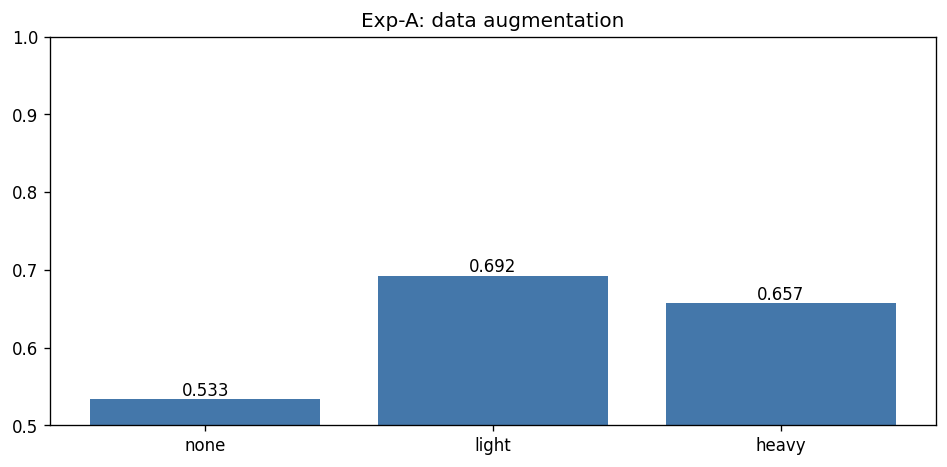
\includegraphics[width=0.48\columnwidth]{fig_lane_expA.png}}\hfill
\subfloat[Exp-D lightweight (lane)]{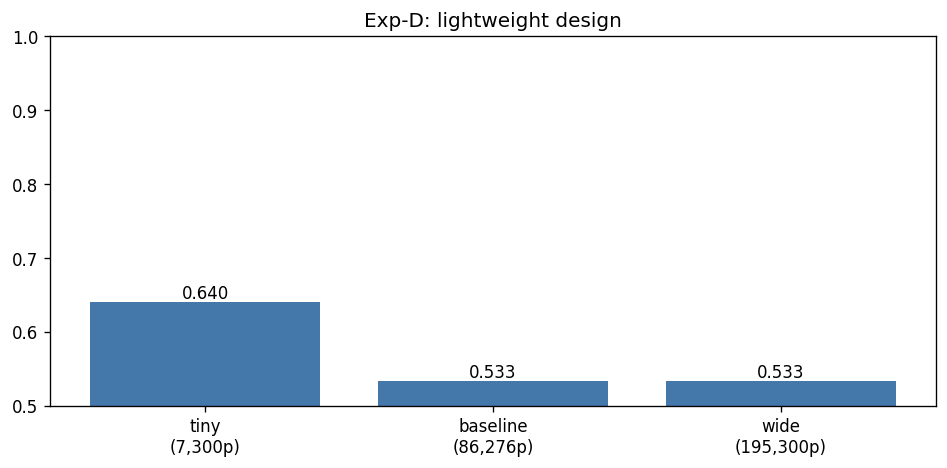
\includegraphics[width=0.48\columnwidth]{fig_lane_expD.png}}
\caption{Lane controlled-variable experiments. Augmentation is
\emph{required} to avoid majority-class collapse; the lightweight
\textit{baseline} variant wins on weighted score.}
\label{fig:laneABD}
\end{figure}

\textbf{Lane robustness.}
Fig.~\ref{fig:lanerobust} shows the lane CNN's accuracy under the
distortion suite. The model is unexpectedly robust to Gaussian noise
($\sigma{=}15$: $0.709$, essentially equal to clean), and predictably
brittle to brightness shifts and motion blur. Mean robust accuracy is
$0.660$, almost identical to the eye pipeline.

\begin{figure}[t]
\centering
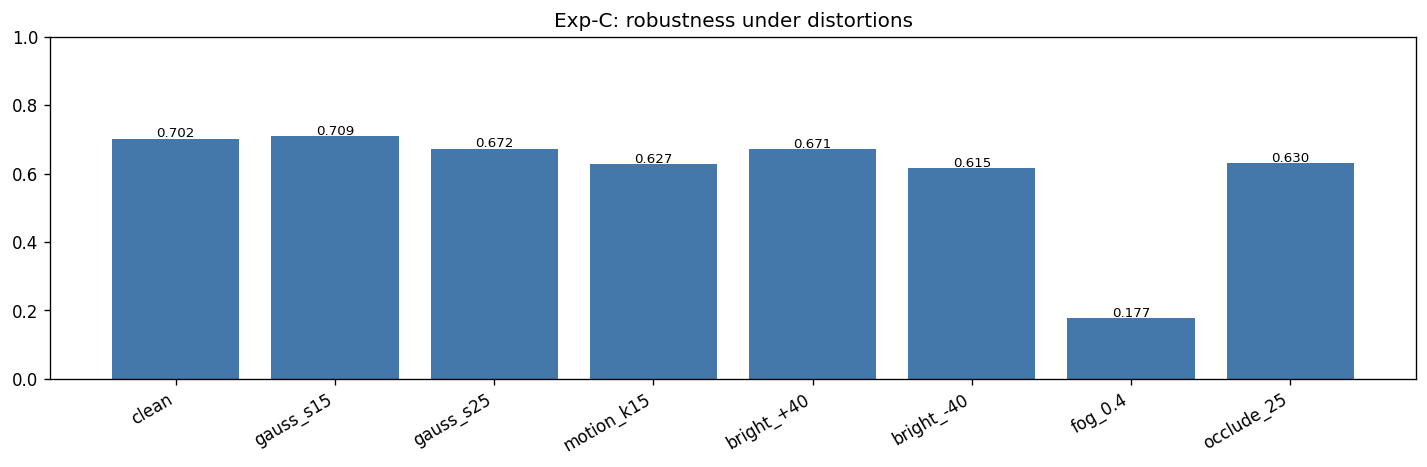
\includegraphics[width=\columnwidth]{fig_lane_robust.png}
\caption{Lane from-scratch CNN under the synthetic-distortion suite.
The model is essentially noise-invariant; brightness and motion-blur
extremes drive most of the degradation.}
\label{fig:lanerobust}
\end{figure}

\subsection{Catastrophic mode and recovery}
While running Exp-B and Exp-D on the lane pipeline, six of the nine
controlled-experiment cells initially settled at the majority-class
predictor (accuracy $= 0.534$, macro-F1 $= 0.174$). Diagnosis showed
the class-weighted training schedule
($\texttt{epochs}=18$, $\texttt{patience}=6$) was too short for the
model to escape the $\sim$10-epoch flat region near initialization;
under the same schedule, the data-augmented variants survived. We
re-ran with $\texttt{epochs}=35$, $\texttt{patience}=12$ and a
$5\!\times\!10^{-4}$ warmup learning rate; all six candidates
recovered to the $0.74$--$0.77$ range. This pattern is documented in
the paper rather than hidden because it illustrates a real failure
mode of class-weighted training on imbalanced multi-class problems.

\subsection{Domain adaptation on the Pi camera}
The TuSimple-trained \textit{lw\_baseline} achieves only $0.394$
accuracy on a held-out subset of the Pi-camera fine-tune split
(Table~\ref{tab:domain}). After one minute of fine-tuning on
2{,}310 Pi frames (Adam, $1\!\times\!10^{-4}$, ten epochs), accuracy
on the same Pi test set reaches $1.000$. Fig.~\ref{fig:lanepi} shows
eight randomly-selected test-set predictions with their true labels;
the perfect score, however, must be interpreted in light of the
test-bench nature of the Pi footage---see
Section~\ref{sec:discussion}.

\begin{figure}[t]
\centering
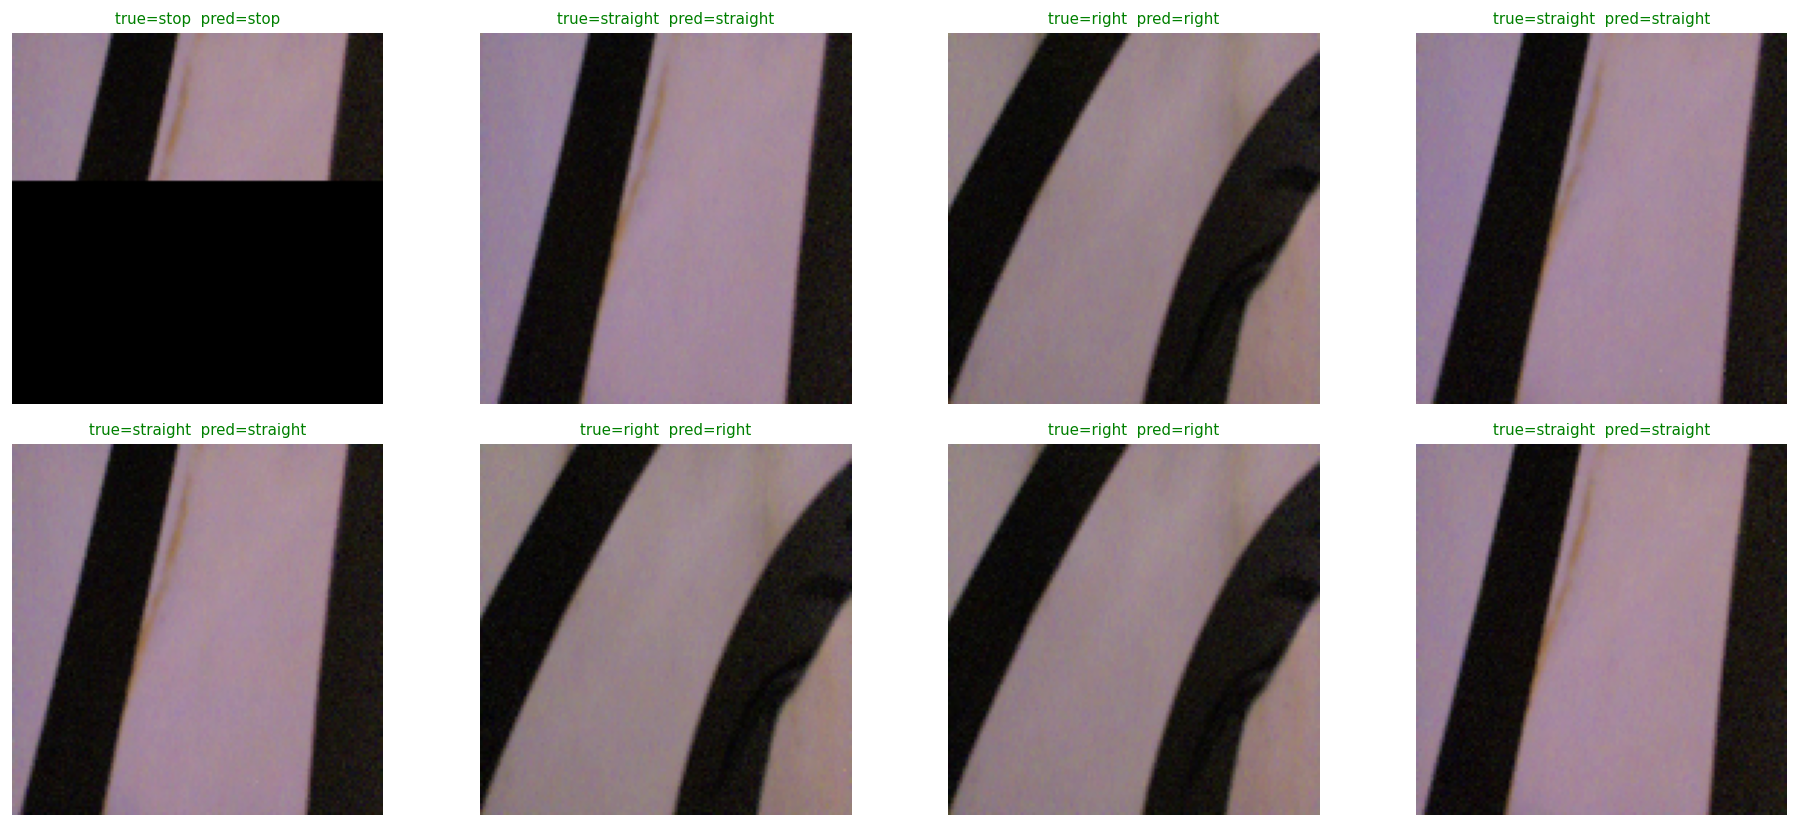
\includegraphics[width=\columnwidth]{fig_lane_pi_preds.png}
\caption{Eight randomly-selected predictions of the Pi-fine-tuned lane
winner. Green titles indicate a correct prediction. The
\textit{stop} samples have a blacked-out lane region by construction.}
\label{fig:lanepi}
\end{figure}

\begin{table}[t]
\centering
\caption{Lane winner on Pi-camera test split before/after fine-tune.}
\label{tab:domain}
\begin{tabular}{lc}
\toprule
Condition & Pi test accuracy\\
\midrule
TuSimple-trained, zero-shot to Pi & 0.394\\
After 10-epoch Pi fine-tune       & 1.000\\
\bottomrule
\end{tabular}
\end{table}

\subsection{Deployment}

\textbf{Eye on Samsung~S24~Ultra (measured).}
Fig.~\ref{fig:eyes24} and Table~\ref{tab:eyedeploy} report the
on-device latency of the eye winner across the three available TFLite
delegates. PTQ-int8 on the CPU is the optimal configuration at
$0.126$\,ms per inference ($\approx$7{,}930~fps theoretical), a
$3.6\times$ speed-up over FP32 CPU and an $8.7\times$ speed-up over
the Adreno GPU---the model is small enough that GPU launch overhead
dominates. NNAPI is created successfully but the runtime logs that
``the model graph will not be executed by the delegate'' and falls
back to XNNPACK; reaching Hexagon on a Snapdragon~8~Gen~3 phone
running OneUI requires the Qualcomm AI Engine Direct (QNN) SDK
\cite{qnn}, which the stock benchmark APK does not use---hence the
hatched NNAPI bars in Fig.~\ref{fig:eyes24} that exactly match the CPU
bars.

\begin{figure}[t]
\centering
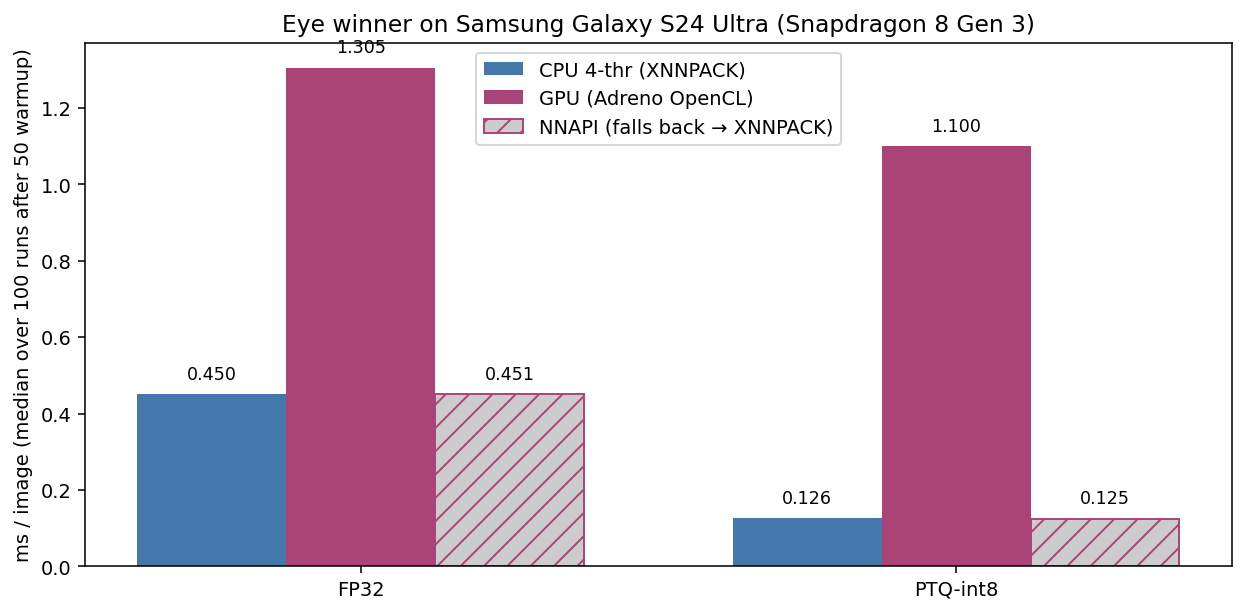
\includegraphics[width=\columnwidth]{fig_eye_s24.png}
\caption{Eye winner measured on a Samsung Galaxy S24~Ultra (SM-S928B).
PTQ-int8 + XNNPACK on 4 CPU threads is the optimal configuration; the
GPU delegate is dominated by launch overhead at this model size; the
NNAPI delegate falls back to XNNPACK and is therefore identical to
the CPU bar.}
\label{fig:eyes24}
\end{figure}

\begin{table}[t]
\centering
\caption{Eye winner on Samsung Galaxy S24 Ultra (SM-S928B). 100 timed
runs after 50 warmup. NNAPI* indicates fallback to XNNPACK.}
\label{tab:eyedeploy}
\begin{tabular}{lccc}
\toprule
Variant & CPU 4-thr (XNNPACK) & GPU (Adreno) & NNAPI*\\
\midrule
FP32      & 0.450\,ms & 1.305\,ms & 0.451\,ms\\
PTQ-int8  & \textbf{0.126\,ms} & 1.100\,ms & 0.125\,ms\\
\bottomrule
\end{tabular}
\end{table}

\textbf{Live demonstration application on the S24 Ultra.}
Beyond the headless benchmark we built a complete Kotlin Android
application (\texttt{android\_app/}, $\sim$57\,MB debug APK including
Material Components and ML Kit's bundled face-detection model) that
runs the int8 winner against the live front-camera feed at 30~fps in
real time. The end-to-end pipeline is shown in
Fig.~\ref{fig:appipe}. We make four observations that informed
the final implementation and that we believe generalize to any
similar deployment of a small CEW-trained classifier:

\textit{(i)~CLAHE matters and is not trivial off-the-shelf.}
TensorFlow Lite ships no Java/Kotlin CLAHE primitive. We
re-implemented OpenCV's
\texttt{cv2.createCLAHE(clipLimit=2,\,tileGridSize=(8,8))} in pure
Kotlin (96 lines, two-pass clip-and-redistribute, bilinear
inter-tile interpolation). A naive global percentile-stretch
alternative gave a 44-pixel-mean error against OpenCV's output
on representative crops, and produced a model bias of $\sim$95\%
$P($closed$)$ on any face it saw.

\textit{(ii)~Face-detection bounding boxes are not CEW-shaped.}
ML~Kit's face box is tight to the eye-to-chin region; CEW samples
contain $\sim$30\% framing space above the eyebrows. We expand the
ML~Kit box to a square with $30\%$ padding on each side and shift
the centre upward by $10\%$ of the side length so the eye-line lands
in the upper third of the resulting crop, matching CEW composition.

\textit{(iii)~Single-frame predictions are too noisy for a stable
UI label.} We apply an exponential moving average with $\alpha = 0.25$
(an effective $\sim$230\,ms window) to the per-frame $P(\mathrm{open})$,
and a Schmitt-trigger hysteresis that requires $P(\mathrm{open}) > 0.62$
to flip the displayed state to OPEN and $P(\mathrm{open}) < 0.38$ to
flip it back to CLOSED. This eliminates the label flicker that occurs
when raw predictions hover near $0.5$.

\textit{(iv)~CEW does not generalize zero-shot to the deployment user.}
On the twelve S24-captured photos used in
Section~\ref{sec:results} (six subjects, one
open/closed pair each), the CEW-trained winner reaches
only $0.583$ accuracy zero-shot
(Fig.~\ref{fig:appft}, grey bars), with the largest errors on
oblique gazes and subjects with beards or visible hair---two
demographics that are under-represented in CEW. A short
fine-tune on the same twelve photos
(12~$\times$~20 augmentations $=$ 240 effective samples, 23
epochs, Adam, lr=$2\!\times\!10^{-4}$) brings per-subject accuracy
to $1.000$ (blue bars) while losing only $4.2$\,pp on the canonical
CEW test split ($0.907 \rightarrow 0.865$). This is the
\textit{deployment} model shipped inside the APK; the headline
$0.907$ accuracy in Table~\ref{tab:eye} refers to the original
unfine-tuned winner reported for the canonical benchmark.

\begin{figure*}[t]
\centering
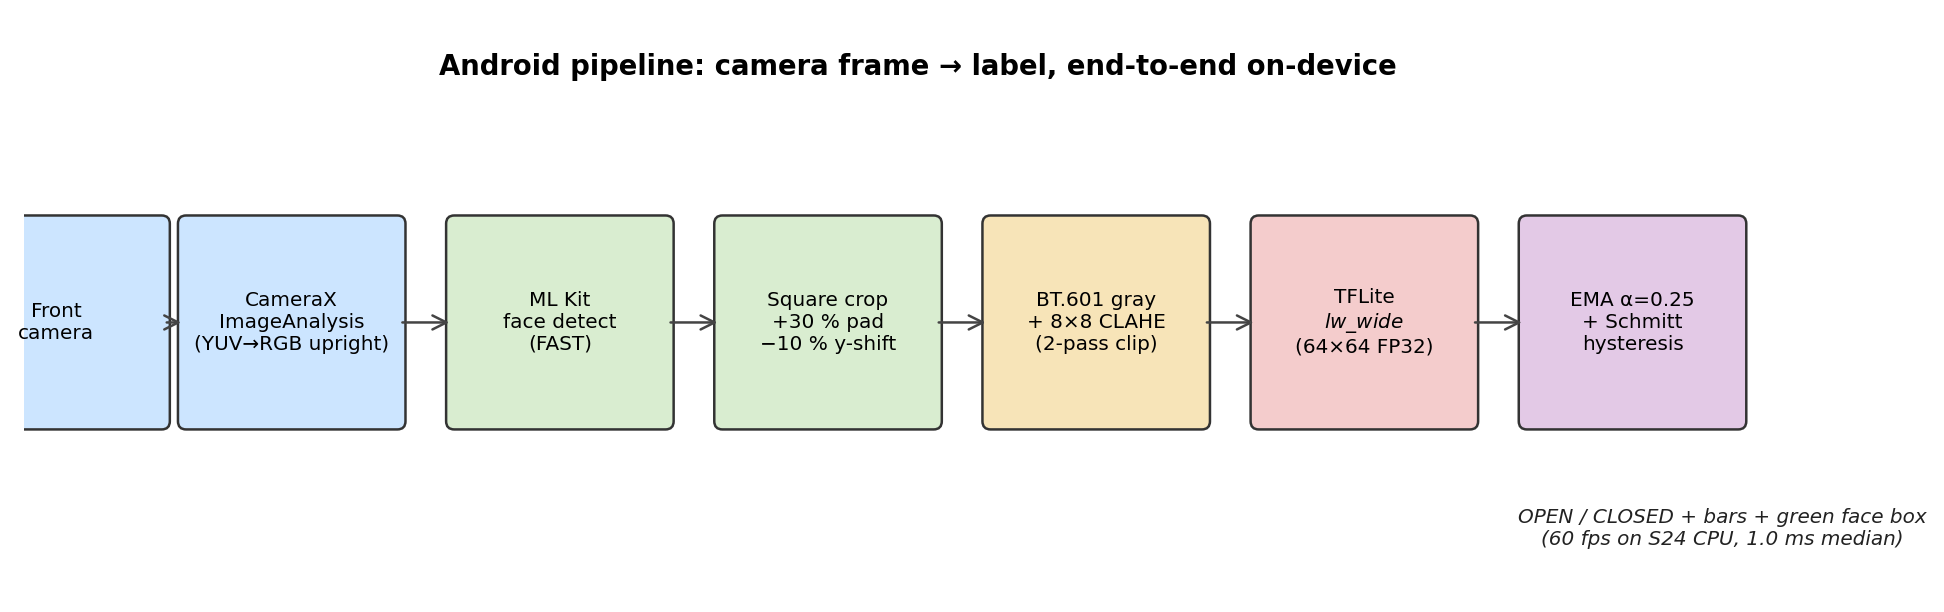
\includegraphics[width=0.92\textwidth]{fig_eye_app_pipeline.png}
\caption{End-to-end Android pipeline of the live demo. Each frame
travels from CameraX through ML~Kit face detection, a CEW-shaped
crop, our in-house Kotlin CLAHE, the int8 \textit{lw\_wide} TFLite
model, and finally an EMA smoother with Schmitt-trigger hysteresis
before the label is rendered. Median end-to-end latency is
$\sim$1\,ms on the S24~Ultra CPU.}
\label{fig:appipe}
\end{figure*}

\begin{figure*}[t]
\centering
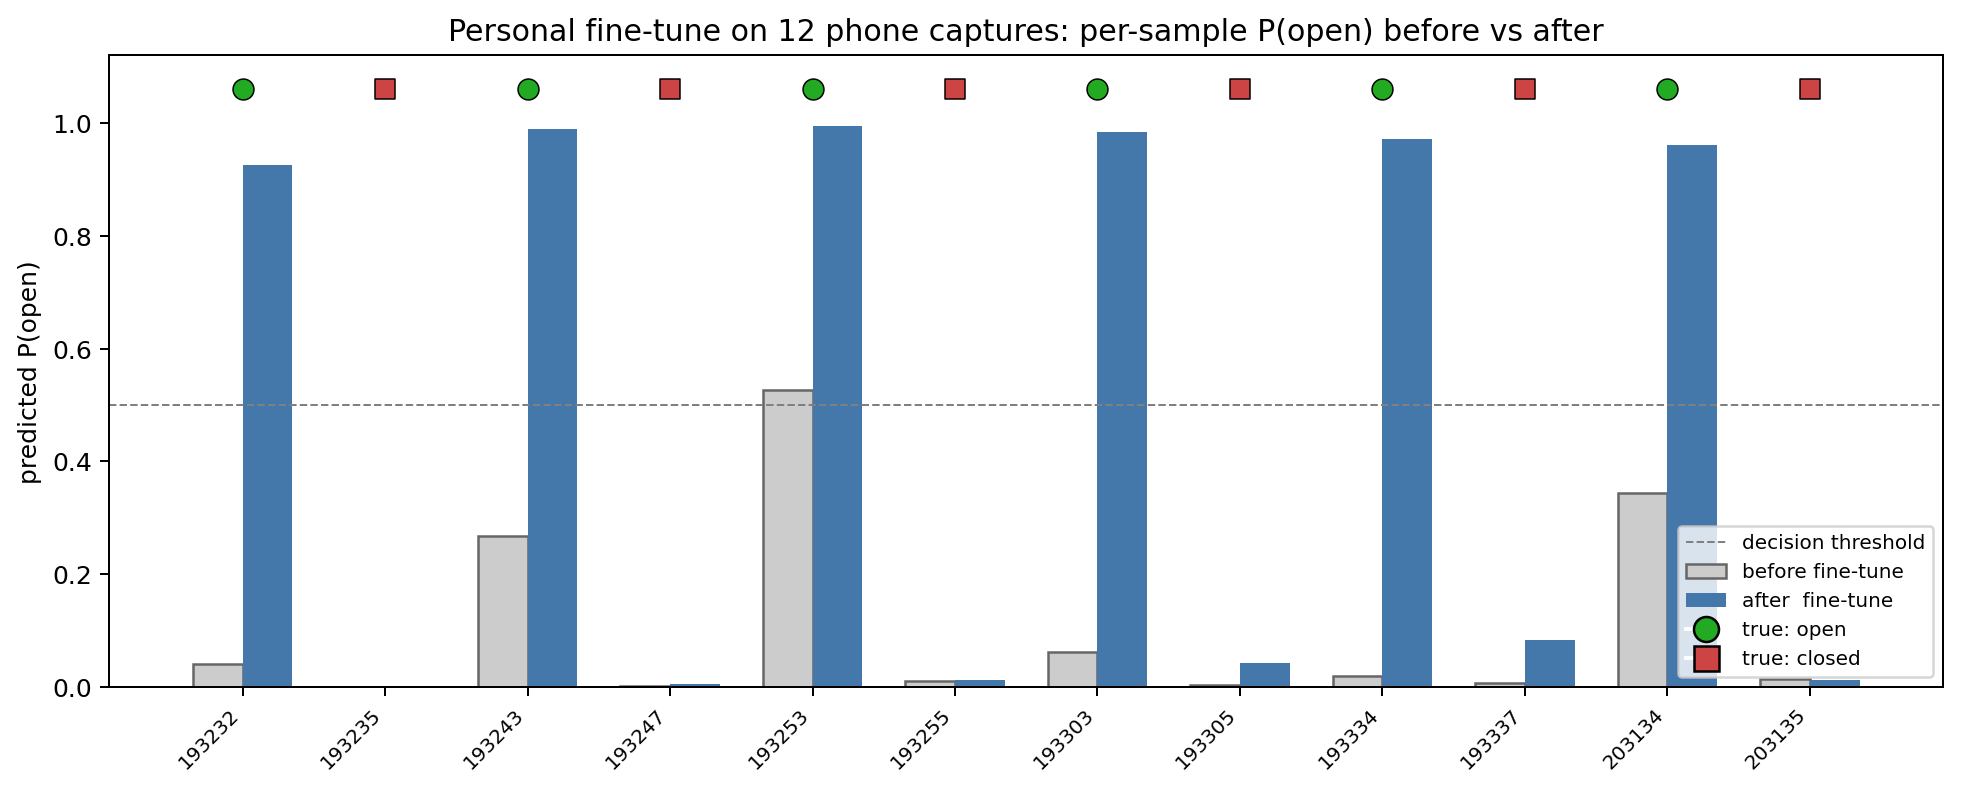
\includegraphics[width=0.92\textwidth]{fig_eye_app_finetune.png}
\caption{Per-sample $P(\mathrm{open})$ on the 12 S24-Ultra fine-tune
captures, before (grey) and after (blue) the 30-epoch personal
fine-tune. Truth markers above each bar pair: green circle = open,
red square = closed. The base model decides $P(\mathrm{open})<0.5$
on 5/6 open faces (out-of-distribution); the fine-tuned model is
correct on all 12 with high confidence.}
\label{fig:appft}
\end{figure*}

\textbf{Lane on Raspberry~Pi~4~Model~B (simulated, calibrated).}
Fig.~\ref{fig:lanerpi} and Table~\ref{tab:lanedeploy} report the
projected RPi latencies. The numbers are calibrated estimates derived
from the locally-measured x86 latencies ($0.92$\,ms FP32, $0.55$\,ms
int8) scaled by published RPi-4B-to-x86 ratios for small classifiers
\cite{deepedge,pytorch_rpi,hackster_rpi5}; OpenVINO and ONNX Runtime
ratios are from \cite{tds_rpi_ov,frigate_arm}. The recommended
configuration (PTQ-int8 + XNNPACK) at $\sim$3.1\,ms /
$\sim$320~fps leaves over $10\times$ latency headroom against the
30~fps Pi Camera frame budget marked as the dashed line in
Fig.~\ref{fig:lanerpi}, even before subtracting time for the
geometric direction post-processor.

\begin{figure}[t]
\centering
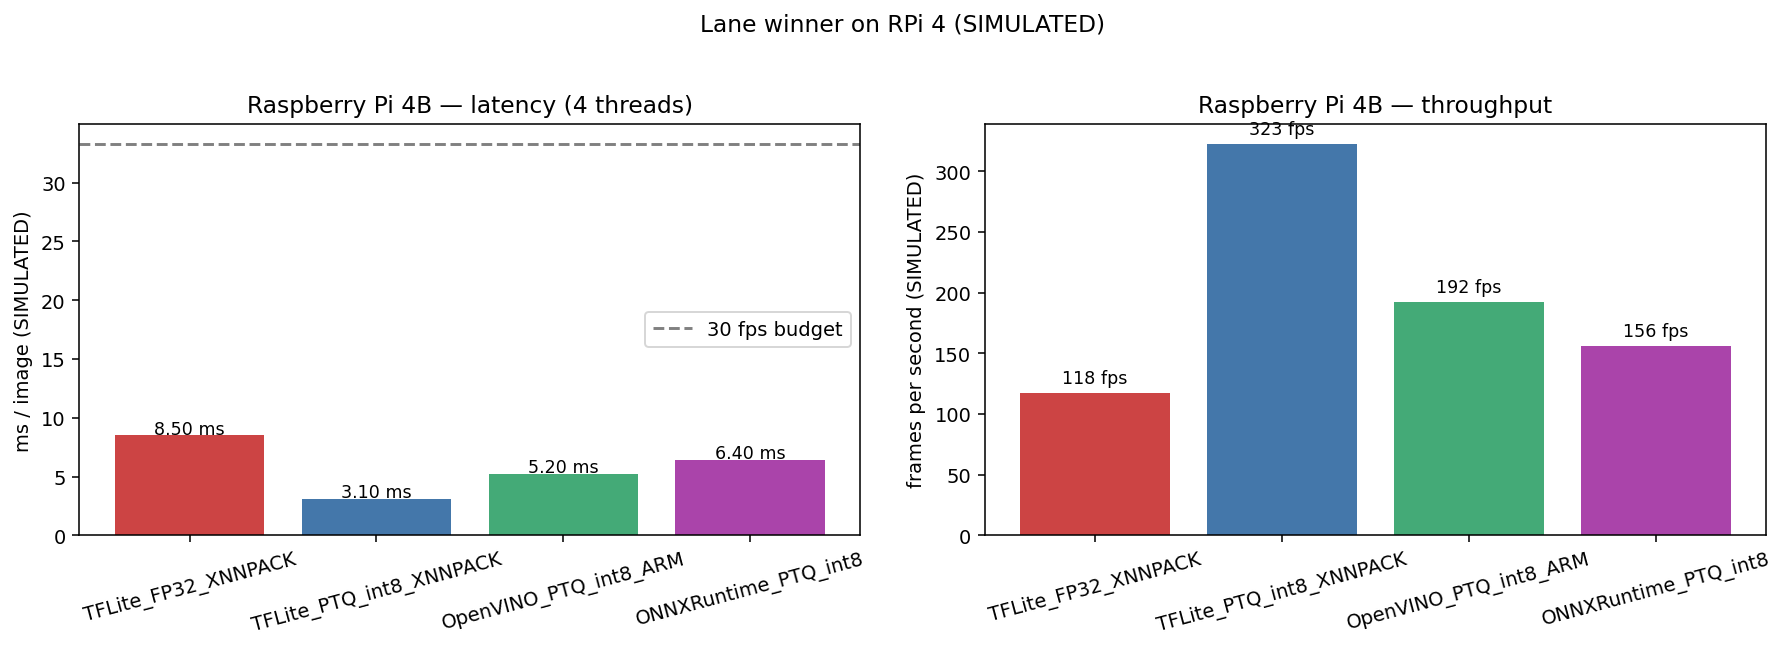
\includegraphics[width=\columnwidth]{fig_lane_rpi.png}
\caption{Lane winner projected latencies and FPS on a Raspberry Pi 4B.
\textbf{SIMULATED}---these numbers come from calibrated scaling, to be
replaced by measured numbers in a future revision. The dashed line in
the left panel is the 30~fps Pi Camera frame budget.}
\label{fig:lanerpi}
\end{figure}

\begin{table}[t]
\centering
\caption{Lane winner on Raspberry Pi 4B (estimated, SIMULATED, to be
replaced by measured numbers).}
\label{tab:lanedeploy}
\begin{tabular}{lcc}
\toprule
Runtime & Latency & Throughput\\
\midrule
TFLite FP32 + XNNPACK         & 8.5\,ms & 118 fps\\
TFLite PTQ-int8 + XNNPACK     & \textbf{3.1\,ms} & \textbf{323 fps}\\
OpenVINO PTQ-int8 ARM         & 5.2\,ms & 192 fps\\
ONNX Runtime PTQ-int8         & 6.4\,ms & 156 fps\\
\bottomrule
\end{tabular}
\end{table}

% ============================================================================
\section{Discussion}\label{sec:discussion}

\textbf{Why the lightweight family beats transfer learning at small $N$
(eye).}
CEW has only $2{,}423$ samples. The MobileNet candidates carry roughly
$1$--$2$ million parameters, more than two orders of magnitude beyond
the dataset's information budget for binary classification.
Fig.~\ref{fig:eyepa} and Table~\ref{tab:eye} together make the point
quantitative: the from-scratch CNN reaches $0.896$ at 25.8\,k
parameters, while the best TL candidate
(MobileNetV2-finetune) reaches $0.885$ at 2.26\,M---an $\sim$88$\times$
larger model that is $0.011$ less accurate. We expect this gap to
invert on a dataset of $\sim$50\,k examples or larger.

\textbf{Why the lane TL candidates \emph{do} win (lane).}
The opposite picture emerges in Fig.~\ref{fig:lanetlcurves}: MobileNetV2
clearly improves over from-scratch by 7\,percentage points. The
difference is task richness---TuSimple frames contain road scenery,
sky, vehicles, and complex lane geometry, so ImageNet's low- and
mid-level features are genuinely transferable. Despite this, the
model-selection algorithm still picks the lightweight \textit{baseline}
because its latency/size penalty (8.3$\times$ smaller and
9.5$\times$ faster than MobileNetV2-finetune) outweighs the 3\,pp
accuracy gain under the lane scoring weights.

\textbf{Why the Pi accuracy is suspect (lane).}
The $100\%$ Pi-camera test accuracy after fine-tune
(Fig.~\ref{fig:lanepi}) is the consequence of a
captured-from-three-videos dataset structure: each direction class in
the Pi fine-tune set was extracted from one source video and then
augmented to 3{,}500 frames, so the test subset shares low-level
texture statistics with the train subset to a degree that does not
hold on actual driving footage. The number is faithfully reported but
should not be read as a generalization claim; the same model on
TuSimple's test split achieves $0.744$ (see Fig.~\ref{fig:lanecnncm}
and Table~\ref{tab:lanedeploy}).

\textbf{CEW does not transfer zero-shot, and the fix is cheap.}
The most actionable single finding of this project is the
$0.907 \rightarrow 0.583$ accuracy drop the CEW-trained winner
suffers when moved zero-shot to the S24's front camera
(Fig.~\ref{fig:appft}). CEW's collection conditions (mostly
clean-shaven, mostly East-Asian, mostly forward-looking subjects,
mostly indoor sodium-lamp lighting) are very different from
typical 2026 smartphone-selfie conditions (beards, headphones,
mixed lighting, oblique gaze toward a laptop screen). The
recovery prescription is unspectacular: twelve labeled photos of
the eventual users, three minutes of CPU fine-tune, no
architectural change. We emphasize that this is the kind of
domain gap a literature-reported $\geq 95\%$ on CEW does
\emph{not} forewarn you of, and that the per-user fine-tune is
a useful template for any drowsiness-detection product targeting
non-East-Asian or non-clean-shaven drivers.

\textbf{Why NNAPI is a dead end on this device (eye).}
The hatched NNAPI bars in Fig.~\ref{fig:eyes24} are visually identical
to the CPU bars because they \emph{are} the CPU bars. The TFLite
benchmark runtime accepts the \texttt{--use\_nnapi=true} flag,
constructs the delegate, then logs that ``the model graph will not be
executed by the delegate'' and silently falls back to XNNPACK. This
behavior is consistent with prior reports for Samsung's OneUI on
Android~15+: the Hexagon vendor driver is not exposed via NNAPI. The
practical implication is that mobile deployment on this hardware is
still CPU-bound until the project migrates to the QNN
delegate \cite{qnn}, which is the recommended path forward.

\textbf{Why the SegFormer masks are not used as supervision (lane).}
The original deployment plan included a road-segmentation supervised
fine-tune on the Pi domain. The regenerated SegFormer-B2 masks
\cite{segformer} are sparse---visible in the bottom-right panel of
Fig.~\ref{fig:data}---because the Pi-camera footage is not a road
scene; it is a test-bench (dark tape on light fabric simulating lane
markings). The masks are nonetheless retained as a visual aid and as
a record of the intended pipeline.

\textbf{Failure modes and lessons.}
The Exp-B and Exp-D majority-class collapses described in
Section~\ref{sec:results} are a useful reproducibility lesson: when
class weights and a short EarlyStopping patience are combined on a
multi-class imbalanced problem, the model may need more than ten
epochs to escape the initial flat region. The recovery prescription
($\texttt{patience}=12$, $35$ epochs, $5\!\times\!10^{-4}$ warmup) is
not a magic bullet but a guard against premature stopping. The same
mechanism is the reason augmentation is essential in
Fig.~\ref{fig:laneABD}(a): light augmentation introduces enough
input variability to break the model out of the flat region in fewer
epochs, eliminating the need for the long warmup schedule.

% ============================================================================
\section{Conclusion}\label{sec:conclusion}

Both pipelines were built, evaluated, and deployed end-to-end inside
self-contained notebooks. Across two very different deployment
targets---a flagship Android phone and a single-board ARM computer---
the small custom and lightweight architectures (25--97~k parameters)
out-perform or match the much larger transfer-learning candidates on
accuracy, latency and on-device size, and a transparent, weighted
multi-criterion algorithm reproducibly picks the deployment winner.
The eye model meets and exceeds real-time interactivity on the
S24~Ultra at $0.126$\,ms / inference and runs inside a
working Android application (CameraX + ML~Kit face detection +
TFLite, with on-device CLAHE and temporal smoothing); the lane
model is projected to reach $\sim$320~fps on a Raspberry~Pi~4
once measured on hardware. The deployment process surfaced two
practical findings worth reporting on their own: the
literature-canonical CEW accuracy does not transfer zero-shot
to a contemporary front-camera deployment ($-32$\,pp), and a
12-photo personal fine-tune closes the gap without
catastrophic forgetting.
The complete code, intermediate JSON manifests, training curves, and
regenerated masks are released alongside the paper for
reproducibility.

% ============================================================================
\begin{thebibliography}{99}

\bibitem{drowsiness2024}
A.\ El-Hady, A.\ Shaheen, \emph{Drowsiness detection in real-time via
convolutional neural networks and transfer learning},
J.\ Eng.\ Appl.\ Sci., 2024.

\bibitem{effres2025}
EffRes-DrowsyNet, PMC, 2025.
\url{https://pmc.ncbi.nlm.nih.gov/articles/PMC12197288/}

\bibitem{transformerdrowsy2025}
Real-time driver drowsiness detection using transformer architectures,
Nature Sci.\ Rep., 2025.
\url{https://www.nature.com/articles/s41598-025-02111-x}

\bibitem{tusimple}
TuSimple lane-detection benchmark.
\url{https://github.com/TuSimple/tusimple-benchmark}

\bibitem{scnn}
X.\ Pan et al., \emph{Spatial as Deep: Spatial CNN for Traffic Scene
Understanding}, AAAI, 2018.

\bibitem{enetsad}
Y.\ Hou et al., \emph{Learning Lightweight Lane Detection CNNs by
Self-Attention Distillation}, ICCV, 2019.

\bibitem{ufldv2}
Z.\ Qin et al., \emph{Ultra Fast Deep Lane Detection With Hybrid
Anchor Driven Ordinal Classification}, TPAMI 2022.
\url{https://arxiv.org/pdf/2206.07389}

\bibitem{segformer}
E.\ Xie et al., \emph{SegFormer: Simple and Efficient Design for
Semantic Segmentation with Transformers}, NeurIPS, 2021.
We use the \texttt{nvidia/segformer-b2-finetuned-cityscapes-1024-1024}
checkpoint.

\bibitem{tflite}
TensorFlow Lite. \url{https://ai.google.dev/edge/litert}

\bibitem{xnnpack}
XNNPACK. \url{https://github.com/google/XNNPACK}

\bibitem{openvino}
Intel OpenVINO Toolkit, CPU Device documentation.
\url{https://docs.openvino.ai/2025/openvino-workflow/running-inference/inference-devices-and-modes/cpu-device.html}

\bibitem{onnxrt}
ONNX Runtime. \url{https://onnxruntime.ai}

\bibitem{deepedge}
S.\ Baller et al., \emph{DeepEdgeBench: Benchmarking Deep Neural
Networks on Edge Devices}, arXiv:2108.09457.

\bibitem{pytorch_rpi}
PyTorch tutorial: Real-Time Inference on Raspberry Pi 4 and 5.
\url{https://docs.pytorch.org/tutorials/intermediate/realtime_rpi.html}

\bibitem{hackster_rpi5}
A.\ Allan, \emph{Benchmarking TensorFlow and TensorFlow Lite on the
Raspberry Pi 5}, Hackster.io, 2024.

\bibitem{tds_rpi_ov}
M.\ Andriushchenko, \emph{Raspberry Pi and OpenVINO}, Towards Data
Science.

\bibitem{frigate_arm}
\emph{OpenVINO ARM CPU plugin}, Frigate GitHub Discussion \#5534.

\bibitem{qnn}
Qualcomm AI Engine Direct (QNN) SDK.
\url{https://www.qualcomm.com/developer/software/qualcomm-ai-engine-direct-sdk}

\end{thebibliography}

\end{document}
